\documentclass[10pt,journal,compsoc]{IEEEtran} %,compsoc

% the package used are listed below
\usepackage{enumerate} %put a number in front of every paragraph
\usepackage{cite} %
\usepackage{amsmath}
\usepackage{algorithm}
\usepackage{algorithmic}
\usepackage{graphicx}
\usepackage{multirow}
\usepackage{subfigure}
\usepackage{amssymb}
\usepackage{color}
%\usepackage[maxfloats=25]{morefloats}
\hyphenation{op-tical net-works semi-conduc-tor}


\begin{document}

\title{Dynamic Random Testing of Web Services: \\ A Methodology and Evaluation}


\author{Chang-ai~Sun,~\IEEEmembership{Senior Member,~IEEE,}
        Hepeng~Dai,
        Guan~Wang,
        Dave~Towey,~\IEEEmembership{Member,~IEEE,}
        Kai-Yuan~Cai,~\IEEEmembership{Member,~IEEE,}
        and~Tsong Yueh~Chen,~\IEEEmembership{Member,~IEEE,}
\thanks{A preliminary version of this paper was presented at the 36th Annual IEEE Computer Software and Applications Conference (COMPSAC 2012)~\cite{sun2012towards}.}
\thanks{C.-A. Sun, H. Dai, and G. Wang are with the School of Computer and Communication Engineering, University of Science and Technology Beijing, Beijing 100083, China. E-mail: casun@ustb.edu.cn.}% <-this % stops a space
\thanks{D. Towey is with the School of Computing Science, University of Nottingham Ningbo China, Ningbo 315100, China. E-mail: dave.towey@nottingham.edu.cn}
\thanks{K.-Y. Cai is with the School of Automation Science and Electrical Engineering, Beihang University, Beijing 100191, China. E-mail: kycai@buaa.edu.cn.}% <-this % stops a
\thanks{T.Y. Chen is with the Department of Computer Science and Software Engineering, Swinburne University of Technology, Hawthorn VIC 3122, Australia. Email: tychen@swin.edu.au.}
}


\markboth{IEEE TRANSACTIONS ON SERVICES COMPUTING,~submitted}%
{Sun \MakeLowercase{\textit{Sun et al.}}: An Empirical Study on Dynamic Random Testing of Web Services: A Methodology and Evaluation}


\IEEEtitleabstractindextext{
\begin{abstract}
 In recent years, Service Oriented Architecture (SOA) has been increasingly adopted to develop distributed applications in the context of Internet. To develop reliable SOA-based applications, an important issue is how to ensure the quality of web services. In this paper, we propose a dynamic random testing (DRT) technique for web services, which is an improvement of the widely-practiced random testing (RT)\textcolor{blue}{~and partition testing (PT)}. We examine key issues when adapting DRT to the context of SOA, including a framework, guidelines for parameter settings, and a prototype for such an adaptation. Empirical studies are reported where DRT is used to test three real-life web services and mutation analysis is employed to measure the effectiveness. Our experimental results show that, compared with two baseline techniques, namely RT and Random Partition Testing (RPT), DRT demonstrates higher fault-detection effectiveness with a lower test case selection overhead, and the theoretical guidelines of parameter setting for DRT are validated to be effective. The proposed DRT and the prototype provide an effective and efficient approach to testing web services.
\end{abstract}

\begin{IEEEkeywords}
Software Testing, Random Testing, Dynamic Random Testing, Web Service, Service Oriented Architecture.
\end{IEEEkeywords}}

\maketitle

\IEEEdisplaynontitleabstractindextext


\IEEEpeerreviewmaketitle


\section{Introduction}
\label{sec:introduction}

\IEEEPARstart{S}{ervice} oriented architecture (SOA)~\cite{papazoglou2008service} defines a loosely coupled, standard-based, service-oriented application development paradigm in the context of Internet. Within SOA, three key roles are defined, namely service providers which develop and own services, service requestors which consume or invoke services, and service registry which registers services from service providers and return services to service requestors. In this context, applications are built upon services that expose functionalities by publishing their interfaces in appropriate repositories, and abstracting entirely from the underlying implementation. Published interfaces may be searched by other services or users and then invoked. web services are the realization of SOA based on open standards and infrastructures~\cite{sun2011transaction}. Ensuring the reliability of SOA-based applications becomes crucial particularly when such applications implement important business processes.

Software testing is a practical method to guarantee quality and reliability of software. However, some features of SOA pose challenges for testing web services~\cite{bartolini2009whitening, canfora2006service}. For instance, service requestors often cannot access the source code of web services which are published and owned by another organization, and as a consequence white-box testing techniques become inapplicable. Therefore, testers naturally turn to black-box testing techniques.

Random Testing (RT)~\cite{Hamlet02} is one of the most widely-practiced black-box testing techniques. In RT, test cases are randomly selected from the input domain (which refers to the set of all possible inputs of the software under test). Therefore, RT is easy to use. Nevertheless, RT may be inefficient in some situations because it does not make use of any information about software under test (SUT) and test history. In recent years, many efforts have been made to improve to RT in different ways~\cite{cai2009random, chen2010adaptive, kuo2007enhanced, Cai07}. For example, adaptive random testing (ART)\textcolor{blue}{~\cite{chen2009adaptive, chen2010adaptive, chen2013code, chen2018test}} is proposed to improve RT in order to make more diverse distribution of test cases in the input domain.

Different from RT, partition testing (PT) aims to generate test cases in a more ``systematic'' way, hopefully using fewer test cases reveal more faults. Firstly, the input domain of SUT divided into disjoint partitions. Then test cases are selected from each and every partition. In PT, each partition is expected to have a certain degree of homogeneity, that is, test cases in same partition should have similar software execution behavior. Ideally, a partition should be homogeneous in fault detection. In other words, if one input is fault-revealing/non-fault-revealing, all other inputs in the same partition shall be fault-revealing/non-fault-revealing too.

RT and PT are based on different intuitions, and they have their own advantages and disadvantages. It is likely that they can be complementary to each other in detecting different faults. Therefore, it is intuitively appealing to investigate the integration of RT and PT. Cai et al.~\cite{cai2009random} have proposed the so-called random partition testing (RPT). In RPT, the input domain is first divided into $m$ partitions $s_1, s_2, \ldots, s_m$, and each $s_i$ is allocated a probability $p_i$. A partition $s_i$ is randomly selected according to the testing profile $\{ \left \langle s_1,p_1 \right \rangle, \left \langle s_2,p_2 \right \rangle, \ldots, \left \langle s_m,p_m \right \rangle\}$, where $p_1 + p_2 + \cdots + p_m = 1$. A concrete test case is then randomly selected from the chosen $s_i$.

In traditional RPT testing, the partitions and corresponding testing profile remain constant during software testing, which may not be a good strategy. Independent researchers from various areas have individually made the same observation that the fault-revealing inputs tend to cluster into ``continuous regions''~\cite{Ammann88, Finelli91}, that is, the similarity of execution behavior among neighboring software inputs. Following the idea of software cybernetics, Cai et al. proposed dynamic random testing (DRT)~\cite{cai2009random}, which is to improve RT and RPT. Different from the original RPT, where the values of $p_i$ are fixed and kept static along the testing process, DRT attempts to dynamically change the values of $p_i$: If a test case from a partition $s_i$ reveals a fault, the corresponding $p_i$ will be increased by a constant $\varepsilon$; otherwise, decreased by the $\varepsilon$.

In practice, web services have been somehow tested at the side of service providers. Those simple or easy-to-test faults are removed and the remaining faults are normally hard to detect. To pursue a higher reliability of web services, simple RT strategy may not be an appropriate candidate technique, especially when the scale of web services is huge or there are some stubborn faults. Some studies show that DRT can improve RT in term of fault detection effectiveness~\cite{Lv2011, Yang2014Dynamic, li2015}.

In this paper, we present a dynamic random testing (DRT) for web services, which is an enhanced version of RT and in the meanwhile an adaptation of DRT to the context of SOA. We further examine key issues of such an adaption, and conduct empirical studies to evaluate the feasibility and effectiveness of the proposed DRT. Experimental results show that DRT evidently outperforms RT. The contributions of this work include:

\begin{itemize}
  \item We develop an effective and efficient testing technique for web services, including a DRT framework which addresses key issues to testing web services and a prototype which partially automates the framework.
  \item We evaluate the performance of DRT through a series of empirical studies on three real web services. It has shown that DRT has significantly higher fault-detection effectiveness than random testing and random partition testing, while its test case selection overhead is lower.
  \item We provide the guidelines of parameter settings of DRT supported by theoretical analysis, and the guidelines are also validated by the empirical studies.
\end{itemize}

The remaining of the paper is organized as follows. Section~\ref{sec:background} introduces the underlying concepts of DRT, web services and mutation analysis. Section~\ref{sec:DRTforwebserivce} presents a framework DRT for web services, guidelines for parameter settings in DRT, and a prototype which partially automates the DRT. Section~\ref{sec:empiricalstudy} describes an empirical study where the proposed DRT is used to test three real-life web services, the results of which are summarized in Section~\ref{sec:results}. Section~\ref{sec:relatedwork} discusses related work and Section~\ref{sec:conclusion} concludes the paper.

\section{Background}
\label{sec:background}

In this section, we present the underlying concepts of DRT, web services, and mutation analysis.

\subsection{Dynamic Random Testing(DRT)}
\label{sec:DRTStrategy}

DRT combines RT and partitioning testing [31] in order to enjoy the benefits of both testing techniques. Assume the test suite \emph{TS} is classified into $m$ partitions denoted as $s_1, s_2, \ldots, s_m$, and suppose that a test case from $s_i$ ($i = 1, 2, \ldots, m$) is selected and executed. If this test case reveals a fault, $\forall j = 1, 2, \ldots, m$ and $j \neq i$, we set

\begin{equation}
\label{eq:DRThitJ}
%\text{new} p_j =
p'_j =
\begin{cases}
p_j - \displaystyle\frac{\varepsilon}{m-1} & \text{if } p_j \geq \displaystyle\frac{\varepsilon}{m-1} \\
0 & \text{if } p_j < \displaystyle\frac{\varepsilon}{m-1}
\end{cases},
\end{equation}

and then

\begin{equation}
\label{eq:DRThitI}
  p'_i = 1 - \sum_{\substack{j = 1 \\ j \neq i}}^m p'_j.
\end{equation}

Otherwise, if the test case does not reveal a fault, we set

\begin{equation}
\label{eq:DRTmissI}
%\text{new } p_i =
p'_i =
\begin{cases}
p_i - \varepsilon & \text{if } p_i \geq \varepsilon \\
0 & \text{if } p_i < \varepsilon
\end{cases},
\end{equation}

and then for $\forall j = 1, 2, \ldots, m$ and $j \neq i$, we set

\begin{equation}
\label{eq:DRTmissJ}
%\text{new } p_j =
p'_j =
\begin{cases}
p_j + \displaystyle\frac{\varepsilon}{m-1} & \text{if } p_i \geq \varepsilon \\
p_j + \displaystyle\frac{p'_i}{m-1} & \text{if } p_i < \varepsilon
\end{cases}.
\end{equation}

The detailed algorithm of DRT is given in Algorithm 1. In DRT, the first test case is selected from a partition that is randomly selected according to the initial probability profile $\{p_1, p_2, \ldots, p_m\}$ (Lines 2 and 3 in Algorithm~\ref{alg:DRT}). After the execution of a test case, the testing profile $\{ \left \langle s_1,p_1 \right \rangle, \left \langle s_2,p_2 \right \rangle, \ldots, \left \langle s_m,p_m \right \rangle\}$ will be updated through changing the values of $p_i$: If a fault is revealed, Formulae~\ref{eq:DRThitJ} and~\ref{eq:DRThitI} will be used; otherwise, Formulas~\ref{eq:DRTmissJ} and~\ref{eq:DRTmissI} will be used. The updated testing profile will be used to guide the random selection of the next test case (Lines 8). Such a process is repeated until the termination condition is satisfied (refer to Line 1). The termination condition here can be either ``testing resource has been exhausted", or ``a certain number of test cases have been executed", or ``a certain number of faults have been detected", etc.

\begin{algorithm}
    \caption{DRT}
    \label{alg:DRT}
    \begin{algorithmic}[1]
        \renewcommand{\algorithmicrequire}{\textbf{Input:}} %ʹ��ԭ���������ж��������\REQUIRE ��\ENSURE��ʾΪInput:��Output:
	    \renewcommand{\algorithmicensure}{\textbf{Output:}}
        \renewcommand{\algorithmicendwhile}{\algorithmicend\_\algorithmicwhile}
		\renewcommand{\algorithmicendfor}{\algorithmicend\_\algorithmicfor}
		\renewcommand{\algorithmicendif}{\algorithmicend\_\algorithmicif}
		\renewcommand{\algorithmicthen}{}
		\renewcommand{\algorithmicdo}{}
        \REQUIRE $\varepsilon, p_1, p_2, \ldots, p_m$
        \WHILE {termination condition is not satisfied}
        \STATE Select a partition $s_i$ according to the testing profile $\{ \left \langle s_1,p_1 \right \rangle, \left \langle s_2,p_2 \right \rangle, \ldots, \left \langle s_m,p_m \right \rangle\}$.
        \STATE Select a test case $t$ from $s_i$.
        \STATE Test the software using $t$.
        \IF {a fault is revealed by $t$}
        \STATE Update $p_j$ ($j = 1, 2, \ldots, m$ and $j \neq i$) and $p_i$ according to Formulae~\ref{eq:DRThitJ} and~\ref{eq:DRThitI}.
        \ELSE
        \STATE Update $p_j$ ($j = 1, 2, \ldots, m$ and $j \neq i$) and $p_i$ according to Formulas~\ref{eq:DRTmissI} and ~\ref{eq:DRTmissJ}.
        \ENDIF
        \ENDWHILE
    \end{algorithmic}
\end{algorithm}

From Formulae~\ref{eq:DRThitJ} to~\ref{eq:DRTmissI}, we can see that an update of testing profile involves $m$ simple calculations, that is, it requires a constant time. In addition, the selection of $s_i$, the selection and execution of a test case all need a constant time. Simply speaking, the execution time for one iteration in DRT is constant. Therefore, the time complexity for DRT to select $n$ test cases is $O(n)$.


\subsection{Web Services}

A web service is a platform-independent, loosely coupled, self-contained programmable web-enabled application that can be described, published, discovered, coordinated and configured using XML artifacts for the purpose of developing distributed interoperable applications~\cite{papazoglou2008service}. A web service consists of description which is usually specified in WSDL, and implementation which can be written in any programming language. web services expose their functionalities by publishing interfaces and at run-time are usually deployed in a service container. In order to invoke a web service, one needs to analyze the input message of its WSDL and assign the expected values.

Web service is a basic component of SOA software. The adoption of SOA, in addition to changing the architecture of a system, brings changes in the process of building the system and using it, and this has effects on testing too~\cite{canfora2006service}.

\begin{itemize}
  \item \emph{lack of observability of the service code and structure:} users and service registry only get interfaces of services, which prevents white-box testing approaches.
  \item \emph{dynamicity and adaptiveness:} For SOA, testers may not be able to determine the component invoked, or the set of possible targets.
  \item \emph{lack of control:} For traditional software testing, testers can control components under test. However, only the services provider has control over the service.
  \item \emph{lack of trust:} A service provider may lie or provide incorrect/inaccutrate description of a service's functional and non-functional behavior, which makes the testing task be difficult.
\end{itemize}

Obviously, SOA testing is more difficult than testing traditional software. RT is a widely used software testing technology, but because of the characteristics of the RT itself, it may not be efficient in web services.

\subsection{Mutation analysis}

Mutation analysis~\cite{demillo1978hints} is widely used to assess the adequacy of test suites and the effectiveness of testing techniques. It applies some mutation operators to seed various faults into the program under test, and thus generates a set of variants, namely mutants. If a test case causes a mutant to show a behavior different from the program under test, we say that this test case ``kills'' the mutant and thus detects the fault injected into the mutant. We normally use the mutation score (MS) to measure how thoroughly a test suite ``kills'' the mutants, which is defined as

\begin{equation}
MS(p,ts) = \displaystyle\frac{N_k}{N_m - N_e}
\end{equation}

where $p$ refers to the program being mutated, $ts$ refers to test suite under evaluation, $N_k$ refers to the number of killed mutants, $N_m$ refers to the total number of mutants, and $N_e$ refers to the number of equivalent mutants. An equivalent mutant refers to one whose behaviors are always the same as those of $p$. It has been pointed out that compared with manually seeded faults, the automatically generated mutants are more similar to the real-life faults, and the mutant score is a good indicator for the effectiveness of a testing technique~\cite{andrews2005mutation}. In this paper, we will use mutation analysis technique to evaluate the effectiveness of the proposed DRT for web services.

\section{Dynamic Random Testing for Web Services}
\label{sec:DRTforwebserivce}

We describe a framework of applying DRT to web services, discuss guidelines for parameter settings in DRT, and present a prototype which partially automates the DRT for web services.

\subsection{Framework}
\label{sec:framework}
Considering the principle of DRT and the features of web services, we propose a framework of DRT for web services, as illustrated in Figure~\ref{fig:frame}. Components in the box are relevant to DRT, and web services under test are located out of the box. The interactions between DRT components and web services are depicted in the framework. We next discuss components in the framework individually.

\begin{figure}[htb]
  \centering
  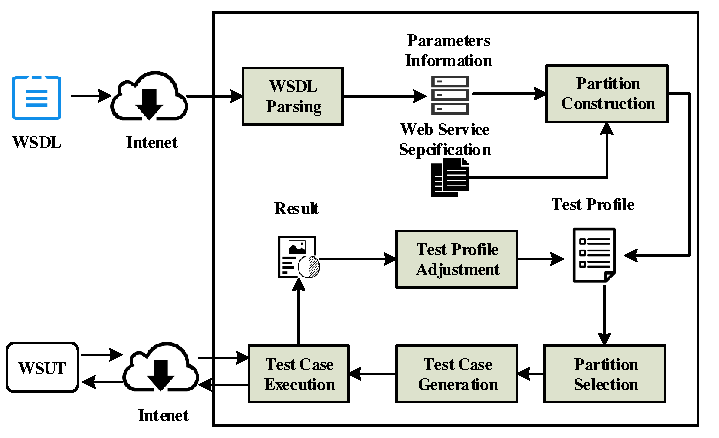
\includegraphics[width = 0.5\textwidth]{fig//framework}
  \caption{The framework of DRT for web services}
  \label{fig:frame}
\end{figure}

\begin{enumerate}[1]
  \item \emph{WSDL Parsing}. web services are composed of services and relevant WSDL document. By parsing the WSDL document, we can get input information for each operation in the services, including the number of parameters, parameter names, parameter types, and additional requirements related to the input parameters.
  \item \emph{Partition Construction}. Partition testing refers to a class of testing techniques~\cite{weyuker1991analyzing}. Although existing partitioning schema may vary from statement, dataflow, branch, path, functionality to risk, we prefer partitions at the specification level to ones at the program level, because DRT is a kind of black-box testing technique combining random testing and partition testing. The principles on achieving convenient and effective partitions have been discussed in some literature~\cite{weyuker1991analyzing, cai2005partition, chen1994relationship, chen1996expected}. According to the specification of web service under test (WSUT) and parameters parsed, we can choose an appropriate method to partition the input domain of WSUT. After partitioning, the testers can assign probability distribution partitions as the initial testing profile. There are different ways to set the initial testing profile. One is to make a uniform probability distribution; the other is to set larger probabilities for those core partitions while smaller probabilities for less important ones.
  \item \emph{Partition Selection}. When the DRT starts, the component is responsible for selecting a partition randomly according to the testing profile.
  \item \emph{Test Case Generation}. Suppose the partition $s_i$ is selected. We can randomly and independently generate a test case that belongs to $s_i$. Since we have parsed the WSDL document, generating test cases can be automated and not particularly difficult.
  \item \emph{Test Case Execution}. The component receives test case generated by Test Case Generation. During the testing, the component is responsible for converting test cases into input messages, invoking web services through the SOAP protocol, and intercepting the test results (namely output messages).
  \item \emph{Test Profile Adjustment}. After one test is completed, the component decides whether the test passes or fails by comparing the actual output with the expected output. With the evaluation result, Probability Distribution Adjustment accordingly adjusts the probability distribution. In some situation, it may be impossible to decide whether one test succeeds or not (namely the oracle problem), then metamorphic testing~\cite{sun2011} may provide an aid to make decisions.
\end{enumerate}

In general, test case generation in DRT for web services still follows the principle of random testing; on the other hand, the selection of next test case (corresponding to a partition) is in accordance with the probability distribution. In this way, DRT takes both advantages of random testing (easiness) and partition testing (effectiveness). In addition, some components in the framework of DRT for web services can be automated, including Partition Selection, Test Case Generation, Test Case Execution, Test Profile Adjustment. In order to make DRT for web services more efficient and practical, we developed a prototype to be described at section~\ref{sec:prototype}.

\subsection{Guidelines for Parameter Settings}
\label{sec:relation}

Our previous work~\cite{sun2012towards} found that the performance of DRT strategy may be affected by the parameter $\varepsilon$ of DRT strategy and the number of partitions. We further explore their impacts through a theoretical analysis. In order to be mathematically tractable, we make the following assumptions:

\begin{enumerate}[1]
  \item The failure rate $\theta_i$ of each partition $s_i$ ($i = 1, 2, \ldots, m$, and $m > 1$) is unknown, but can be estimated.
  \item The failure rate~$\theta_i$ ($i = 1, 2, \ldots, m$, and $m > 1$)~remains unchanged during the testing process, that is, faults are not removed after detection of failure.
  \item Test cases are selected with replacement, that is, same test cases may be selected more than once.
\end{enumerate}

The main idea of DRT strategy is to increase the selecting probabilities of the partitions that have larger failure rates. Parameter $\varepsilon$ is used to update the testing profile during the testing process, and the number of partitions also affects the speed of updating the testing profile according to Formulae 1 and 3. Therefore, under a certain number of partitions, we are interested in investigating the settings of $\varepsilon$ to achieve better performance of DRT strategy.

We assume that the maximum of all failure rates is $\theta_M$. $s_M$ denotes the partition that has a failure rate $\theta_M$. Let $p_i^n$ denote the probability of after executing the $n^{th}$ test case from partition $s_i$. As the testing proceeds, the probability $p_M$ of partition $s_M$ being selected is expected to be increased, namely
\begin{equation}
\label{eq:exception}
p_M^{n + 1} > p_M^{n}
\end{equation}
At the beginning, the testing profile is~$\{ \left \langle s_1,p_1^0 \right \rangle, \left \langle s_2,p_2^0 \right \rangle, \ldots, \left \langle s_m,p_m^0 \right \rangle\}$. After $n^{th}$ test cases have been executed, the testing profile has updated to~$\{ \left \langle s_1,p_1^n \right \rangle, \left \langle s_2,p_2^n \right \rangle, \ldots, \left \langle s_m,p_m^n \right \rangle\}$. Note that $p_i^n$ is increased/decreased by the parameter $\varepsilon$ during the testing process, and the value of $\varepsilon$ is relatively small. For instance, in~\cite{Lv2011} and~\cite{li2015}, the value of $\varepsilon$ is set 0.05. On the other hand, the initial $p_i^0$ is larger than $\varepsilon$, and the adjustment of $p_i$ is relatively small according to Formulae~\ref{eq:DRThitJ} to~\ref{eq:DRTmissJ}, which rarely leads to the situation~$p_i < \varepsilon / (m - 1)$~or~$p_i < \varepsilon$ ($i = 1, 2, \ldots, m$), so we do not consider this.


Without loss of generality, we explore the relation between $p_i^{n + 1}$ and $p_i^{n}$. We calculate the conditional probability $p(i|\delta)$ of following four cases (denoted as $\delta_1, \delta_2, \delta_3$, and $\delta_4$, respectively).

\begin{enumerate}[ {Case} 1 ($\delta_1$):]
  \item \textbf{$t_{n} \notin s_i$ and a fault is detected by $t_n$}, then $p(i|\delta_1)$ is calculated as follows according to Formula 1:
  \begin{equation}
  p(i|\delta_1) = \sum_{i \neq j}\theta_j(p_i^n - \displaystyle\frac{\varepsilon}{m - 1}).
  \end{equation}
  \item \textbf{$t_{n} \in s_i$ and a fault is detected by $t_n$}, then $p(i|\delta_2)$ is calculated as follows according to Formula 2:
  \begin{equation}
  p(i|\delta_2) = \theta_i(p_i^n + \varepsilon).
  \end{equation}
  \item \textbf{$t_{n} \in s_i$ and no fault is detected by $t_n$}, then $p(i|\delta_3)$ is calculated as follows according to Formula 3:
  \begin{equation}
  p(i|\delta_3) = (1 - \theta_i)(p_i^n - \varepsilon).
  \end{equation}
  \item \textbf{$t_{n} \notin s_i$ and no fault is detected by $t_n$}, then $p(i|\delta_4)$ is calculated as follows according to Formula 4:
  \begin{equation}
  p(i|\delta_4) = \sum_{i \neq j}(1 - \theta_j)(p_i^n + \displaystyle\frac{\varepsilon}{m - 1}).
  \end{equation}
\end{enumerate}
Therefore, we have $p_i^{n + 1}$ for all cases together is as follows:
\begin{equation}
\label{eq:7}
\begin{split}
p_i^{n + 1} = &p_i^n\theta_i(p_i^n + \varepsilon) + p_i^n(1-\theta_i)(p_i^n - \varepsilon)\\
&+ \sum_{j \neq i}p_j^n\theta_j(p_i^n - \displaystyle \frac{\varepsilon}{m- 1})\\
&+ \sum_{j \neq i}p_j^n(1 - \theta_j)(p_i^n + \displaystyle\frac{\varepsilon}{m - 1})\\
=&(p_i^n)^2\theta_i + p_i^n\theta_i\varepsilon + (p_i^n)^2 - p_i^n\varepsilon - (p_i^n)^2\theta_i + p_i^n\theta_i\varepsilon\\
& + (p_i^n - \displaystyle\frac{\varepsilon}{m - 1})\sum_{j \neq i}p_j^n\theta_j + (p_i^n + \displaystyle\frac{\varepsilon}{m - 1})\sum_{j \neq i}p_j^n\\
&- (p_i^n + \displaystyle\frac{\varepsilon}{m - 1})\sum_{j \neq i}p_j^n\theta_j\\
=&(p_i^n)^2 + 2p_i^n\theta_i\varepsilon - p_i^n\varepsilon + (p_i^n - \displaystyle\frac{\varepsilon}{m - 1} - p_i^n \\
&- \displaystyle\frac{\varepsilon}{m - 1})\sum_{j \neq i}p_j^n\theta_j + (p_i^n + \displaystyle\frac{\varepsilon}{m - 1})(1 - p_i^n)\\
=&p_i^n + (p_i^n)^2 - (p_i^n)^2 + 2p_i^n\theta_i\varepsilon - p_i^n\varepsilon + \displaystyle\frac{\varepsilon}{m - 1} - \\
&\displaystyle\frac{\varepsilon}{m - 1}p_i^n - \displaystyle\frac{2\varepsilon}{m - 1}\sum_{j \neq i}p_j^n\theta_j\\
=&p_i^n + \displaystyle\frac{\varepsilon}{m - 1}(2p_i^n\theta_im - p_i^nm - 2p_i^n\theta_i + 1 )\\
&- \displaystyle\frac{2\varepsilon}{m-1}\sum_{j \neq i}p_j^n\theta_j\\
=&p_i^n + Y_i^n,
\end{split}
\end{equation}
where
\begin{equation}
\begin{split}
\label{eq:yi}
Y_i^n = &\displaystyle\frac{\varepsilon}{m - 1}(2p_i^n\theta_im - p_i^nm - 2p_i^n\theta_i + 1 )\\
         &- \displaystyle\frac{2\varepsilon}{m-1}\sum_{j \neq i}p_j^n\theta_j.
\end{split}
\end{equation}
From Formula~\ref{eq:yi}, we have:
\begin{equation}
\begin{split}
\label{eq:26}
Y_M^n - Y_i^n = &\displaystyle\frac{\varepsilon}{m - 1}(2p_M^n\theta_Mm - p_M^nm - 2p_M^n\theta_M + 1)\\
& - \displaystyle\frac{2\varepsilon}{m - 1}\sum_{j \neq M}p_j^n\theta_j - \displaystyle\frac{\varepsilon}{m - 1}(2p_i^n\theta_im - p_i^nm\\
& - 2p_i^n\theta_i + 1) + \displaystyle\frac{2\varepsilon}{m - 1}\sum_{j \neq i}p_j^n\theta_j \\
=&\displaystyle\frac{\varepsilon}{m - 1}(2m(p_M^n\theta_M - p_i^n\theta_i) - m(p_M^n - p_i^n) -\\
& 2(p_M^n\theta_M - p_i^n\theta_i)) - \sum_{j \neq M}p_j^n\theta_j + \sum_{j \neq i}p_j^n\theta_j    \\
=& \displaystyle\frac{2\varepsilon}{m - 1}(m(p_M^n\theta_M - p_i^n\theta_i) - \displaystyle\frac{m(p_M^n - p_i^n)}{2} - \\
&(p_M^n\theta_M - p_i^n\theta_i)) + \displaystyle\frac{2\varepsilon}{m-1}(p_M^n\theta_M - p_i^n\theta_i)\\
=&\displaystyle\frac{2\varepsilon}{m - 1}(m(p_M^n\theta_M - p_i^n\theta_i) - \displaystyle\frac{m(p_M^n - p_i^n)}{2}).
\end{split}
\end{equation}

Before presenting the final guidelines, we need the following lemma first.
\newtheorem{lem}{Lemma}
\label{Lemma}
\begin{lem}
  If $p_i^{n} - p_M^{n} > 2(p_i^{n}\theta_i - p_M^{n}\theta_M)$, then $p_M^{n + 1} > p_M^{n}$.
\end{lem}

\emph{Proof:} The condition $p_i^{n} - p_M^{n} > 2(p_i^{n}\theta_i - p_M^{n}\theta_M)$ can be equivalently expressed as:
\begin{equation}
  \label{lemma:proof1}
\displaystyle\frac{p_M^n - p_i^n}{2} < p_M^{n}\theta_M - p_i^{n}\theta_i.
\end{equation}
From Formula~\ref{lemma:proof1}, we have $(p_M^{n}\theta_M - p_i^{n}\theta_i) - \displaystyle\frac{p_M^n - p_i^n}{2} > 0$. Since $0 < \varepsilon < 1$, and $m > 1$, hence the following formula is true:
\begin{equation}
  \label{lemma:proof2}
\displaystyle\frac{2m\varepsilon}{m - 1}((p_M^{n}\theta_M - p_i^{n}\theta_i) - \displaystyle\frac{p_M^n - p_i^n}{2}) > 0.
\end{equation}
Furthermore, we have:
\begin{equation}
  \label{lemma:proof3}
\displaystyle\frac{2\varepsilon}{m - 1}(m(p_M^{n}\theta_M - p_i^{n}\theta_i) - \displaystyle\frac{m(p_M^n - p_i^n)}{2}) > 0.
\end{equation}

According to Formula \ref{lemma:proof3} and \ref{eq:26}, if $p_i^{n} - p_M^{n} > 2(p_i{n}\theta_i - p_M^{n}\theta_M)$, we have $Y_M^n - Y_i^n > 0$. Directly, $\sum_{i=1}^mY_i^n = 0$, because~$\sum_{i=1}^mp_i^{n + 1} = 1$, and $\sum_{i=1}^mp_i^{n} = 1$. Then, we have $Y_M^n >0$. According to Formula~\ref{eq:7}, we have $p_M^{n + 1} = p_M^n + Y_M^n$. Since $Y_M^n >0$, obviously, $p_M^{n + 1} > p_M^n$. $\hfill{} \Box$

Accordingly, we now present the following theorem that states a sufficient condition to achieve $p_M^{n + 1} > p_M^{n}$.
%\newtheorem{theo}{Theorem}
%\label{theorem}
%\begin{theo}
%  For all failure rates $\theta_i, i \in \{1, 2, \ldots, m\}$, and $\theta_M$ is the maximum of $\theta_i$, the following condition is sufficient to guarantee that $p_M^{n + 1} > p_M^{n}$
%\begin{equation}
%  \displaystyle\frac{1}{4\theta_M\theta_{\Delta}} < \displaystyle\frac{m + \varepsilon}{m\varepsilon} < \displaystyle\frac{1}{2\theta_\Delta}
%\end{equation}

\newtheorem{theo}{Theorem}
\label{theorem}
\begin{theo}
  For failure rate $\theta_{min} = min\{\theta_1, \ldots, \theta_m\}$, $\theta_M > \theta_{min}$, if $0 < \theta_{min} < \frac{1}{2}$, the following condition is sufficient to guarantee that $p_M^{n + 1} > p_M^{n}$:
\begin{equation}
\label{equa:results}
  \displaystyle\frac{2m\theta_{min}^2}{1-2\theta_{min}} < \varepsilon < \displaystyle\frac{(m-1)m\theta_{min}}{2(m + 1)}.
\end{equation}


%where $\theta_i \le \theta_\Delta < \theta_M$, and $\theta_i \ne \theta_M$.
\end{theo}
\emph{proof:} In order to guarantee $p_M^{n + 1} > p_M^{n}$, we consider the following three kinds of cases where $i \in \{1, 2, \ldots, m\}$ and $i \ne M$.

\textbf{Case 1 ($p_i^n = p_M^n$):} Since $\theta_i < \theta_M$, then $(p_i^n\theta_i - p_M^n\theta_M) < 0$. Directly, $(p_i^n - p_M^n) > 2(p_i^n\theta_i - p_M^n\theta_M)$. According to Lemma 1, we have $p_M^{n + 1} > p_M^{n}$.

%\textbf{Case 2 ($p_i^n > p_M^n$):} Since $1/2\theta_\Delta > (m + \varepsilon)/m\varepsilon$, and $1/2\theta_i \ge 1/2\theta_\Delta$, then $(p_i^n - p_M^n)\varepsilon > 2(p_i^n - p_M^n)\theta_i(m + \varepsilon)/m$, and $(p_i^n - p_M^n)\varepsilon > 2(p_i^n - p_M^n)\theta_i$. Because $\theta_M > \theta_i$, we have $2(p_i^n - p_M^n)\theta_i > 2(p_i^n\theta_i - p_M^n\theta_M)$. Then $(p_i^n - p_M^n)\varepsilon > 2(p_i^n\theta_i - p_M^n\theta_M)$. According to Lemma 1, we have $p_M^{n + 1} > p_M^{n}$.

\textbf{Case 2 ($p_i^n > p_M^n$):} According to Formula \ref{equa:results}, we have the following formula:
$$\varepsilon > \displaystyle\frac{2m\theta_{min}^2}{1-2\theta_{min}}.$$
Since
    $$\displaystyle\frac{2m\theta_{min}^2}{1-2\theta_{min}} = \displaystyle\frac{\theta_{min}}{1/2m\theta_{min} - 1/m},$$
we have the following formula:
    $$\varepsilon > \displaystyle\frac{\theta_{min}}{1/2m\theta_{min} - 1/m}.$$
Because $\theta_{min} < 1/2$, we have $1/2m\theta_{min} - 1/m > 0$ and $\varepsilon(1/2m\theta - 1/m) > \theta_{min}$ that is $\varepsilon/2m\theta_{min} > \theta_{min} + \varepsilon/m$.
Because $\varepsilon > 0$, and $m > 1$, then there holds
 $$\displaystyle\frac{1}{2\theta_{min}} > \displaystyle\frac{(\theta_{min} + \varepsilon/m)}{(\varepsilon/m)}.$$
Actually, $(1/2\theta_{min})(p_i^n - p_M^n) > (p_i^n - p_M^n)(\theta_{min} + \varepsilon/m)/(\varepsilon/m)$ as $p_i^n > p_M^n$, and
$$p_i^n -p_M^n > 2\theta_{min}(p_i^n -p_M^n)\displaystyle\frac{\theta_{min} + \varepsilon/m}{\varepsilon/m}.$$
Because $(\theta_{min} + \varepsilon/m)/(\varepsilon/m) > 1$, we have
$$2\theta_{min}(p_i^n -p_M^n)\displaystyle\frac{\theta_{min} + \varepsilon/m}{\varepsilon/m} > 2\theta_{min}(p_i^n -p_M^n).$$
Since $\theta_{min} < \theta_M$, then
$$2\theta_{min}(p_i^n - p_M^n) > 2(p_i^n\theta_{min} - p_M^n\theta_M).$$
Thus,
$$p_i^n -p_M^n > 2(p_i^n\theta_{min} - p_M^n\theta_M).$$
According to Lemma 1, we have $p_M^{n + 1} > p_M^{n}$.
%Furthermore, we have $(1/2\theta_{min})(p_i^n - p_M^n) > (p_i^n - p_M^n)(\theta_{min} + \varepsilon/m)/(\varepsilon/m)$, and $p_i^n - p_M^n > 2(p_i^n - p_M^n)\theta_{min}(\theta_{min} + \varepsilon/m)/(\varepsilon/m)$. Because $2(p_i^n - p_M^n)\theta_{min}(\theta_{min} + \varepsilon/m)/(\varepsilon/m) > 2(p_i^n - p_M^n)\theta_{min}$, and $2(p_i^n - p_M^n)\theta_{min} > 2(p_i^n\theta_{min} - p_M^n)$, we have $(p_i^n - p_M^n) > 2(p_i^n\theta_i - p_M^n\theta_M)$. According to Lemma 1, $p_M^{n + 1} > p_M^{n}$ is satisfied.

%\textbf{Case 3 ($p_i^n < p_M^n$):} Since $1/2\theta_M < (m + \varepsilon)/m\varepsilon$, then $(p_M^n - p_i^n)\varepsilon < 2(p_M^n - p_i^n)\theta_M(m + \varepsilon)/m$. Because $\theta_i < \theta_M$, we have $2(p_M^n - p_i^n)\theta_M(m + \varepsilon)/m < 2(p_M^n\theta_M - p_i^n\theta_i)(m + \varepsilon)/m$. Furthermore, we have $(p_M^n - p_i^n)\varepsilon < 2(p_M^n\theta_M - p_i^n\theta_i)(m + \varepsilon)/m$, and thus $(p_i^n - p_M^n)\varepsilon > 2(p_i^n\theta_i - p_M^n\theta_M)(m + \varepsilon)/m$. According to Lemma 1, we have $p_M^{n + 1} > p_M^{n}$. $\hfill{} \Box$

\textbf{Case 3 ($p_i^n < p_M^n$):}
Before giving proof, we make the following assumption: $\frac{1}{2} < \theta_M < 1$.

Since we have the following formula:
$$\varepsilon < \displaystyle\frac{(m - 1)m\theta_{min}}{2(m + 1)}$$
and
$$\displaystyle\frac{(m - 1)m\theta_{min}}{2(m + 1)} = \displaystyle\frac{2m -(m + 1)}{2(m + 1)}m\theta_{min},$$
thus
$$\varepsilon < (\displaystyle\frac{m}{m +1} - \displaystyle\frac{1}{2})m\theta_{min}.$$
Obviously, $\varepsilon/m < (m/(m + 1) - 1/2)\theta_{min}$ as $m > 1$. Furthermore, we have
$$-\displaystyle\frac{\varepsilon}{m} > (\displaystyle\frac{1}{2} - \displaystyle\frac{m}{m + 1})\theta_{min}$$
and
$$\displaystyle\frac{m\theta_{min}}{m + 1} - \displaystyle\frac{\varepsilon}{m} + \displaystyle\frac{2\varepsilon}{m} > \displaystyle\frac{\theta_{min}}{2} + \displaystyle\frac{2\varepsilon}{m}$$
which subjects to
$$\displaystyle\frac{m\theta_{min}}{m + 1} + \displaystyle\frac{\varepsilon}{m}  > \displaystyle\frac{1}{2}(\theta_{min} + \displaystyle\frac{4\varepsilon}{m}).$$
It easily follows that $(m\theta_{min}/(m + 1) + \varepsilon/m)/(4\varepsilon/m + \theta_{min}) > 1/2$ for any $m > 1, \varepsilon > 0$, and $0 < \theta_{min} < 1$.
Since $\frac{1}{2} < \theta_M < 1$, we have $(m\theta_{min}/(m + 1) + \varepsilon/m)/(4\varepsilon/m + \theta_{min}) > 1/2\theta_M$. Then we have
$$2(p_M^n -p_i^n)\theta_M\displaystyle\frac{\displaystyle\frac{\varepsilon}{m} +\displaystyle\frac{m\theta_{min}}{m + 1}}{\displaystyle\frac{4\varepsilon}{m} + \theta_{min}} > p_M^n -p_i^n$$
as $p_M^n > p_i^n$.
Since $\varepsilon/m < 4\varepsilon/m$, and $m\theta_{min}/(m + 1) < \theta_{min}$, we have
$$ \displaystyle\frac{\displaystyle\frac{\varepsilon}{m} +\displaystyle\frac{m\theta_{min}}{m + 1}}{\displaystyle\frac{4\varepsilon}{m} + \theta_{min}} < 1$$
and
$$ 2(p_M^n -p_i^n)\theta_M > 2(p_M^n -p_i^n)\theta_M\displaystyle\frac{\displaystyle\frac{\varepsilon}{m} +\displaystyle\frac{m\theta_{min}}{m + 1}}{\displaystyle\frac{4\varepsilon}{m} + \theta_{min}}$$
Hence we have
$$2(p_M^n -p_i^n)\theta_M > p_M^n -p_i^n$$
which can be equivalently expressed as
$$p_i^n -p_M^n > 2(p_i^n - p_M^n)\theta_M.$$
Since $\theta_{min} < \theta_M$, we have $2(p_i^n - p_M^n)\theta_M > 2(p_i^n\theta_{min} - p_M^n\theta_M)$, therefore,
$$p_i^n -p_M^n > 2(p_i^n\theta_{min} - p_M^n\theta_M).$$
According to Lemma 1, we have $p_M^{n + 1} > p_M^{n}$. $\hfill{} \Box$


%Since $\varepsilon < (m - 1)m\theta_{min}/2(m + 1)$, and $\varepsilon < (m/(m + 1) - 1/2)m\theta_{min}$, then, $\varepsilon/m < (m/(m + 1) - 1/2)\theta_{min}$, and $-\varepsilon/m > (1/2 - m/(m +1))\theta_{min}$. Furthermore, we have $\varepsilon/m + m\theta_{min}/(m + 1) > 2\varepsilon/m + \theta_{min}/2$, and thus $((\varepsilon/m + m\theta_{min})/(m + 1))/(4\varepsilon/m + \theta_{min}) > 1/2\theta_M$. Because $p_M^n > p_i^n$, we have $2(p_M^n -p_i^n)\theta_M((\varepsilon/m + m\theta_{min}/(m + 1))/(4\varepsilon/m + \theta_{min})) > (p_M^n - p_i^n)$. Since $\varepsilon/m < 4\varepsilon/m$, and $m\theta_{min}/(m + 1) < \theta_{min}$, we have $((\varepsilon/m + m\theta_{min}/(m + 1))/(4\varepsilon/m + \theta_{min})) < 1$, and $2(p_M^n - p_i^n)\theta_M > p_M^n - p_i^n$. Because $2(p_M^n\theta_M - p_i^n\theta_{min}) > 2(p_M^n - p_i^n)\theta_M$, we have $2(p_M^n\theta_M - p_i^n\theta_{min}) > p_M^n - p_i^n$, and $p_i^n - p_M^n > 2(p_i^n\theta_{i} - p_M^n\theta_M)$. According to Lemma 1, $p_M^{n + 1} > p_M^{n}$ is satisfied. $\hfill{} \Box$

To sum up, when $\frac{1}{2} < \theta_M < 1$, there is always an interval $E$:
\begin{equation}
  \varepsilon \in (\displaystyle\frac{2m\theta_{min}^2}{1 - 2\theta_{min}}, \displaystyle\frac{(m - 1)m\theta_{min}}{2(m + 1)})
\end{equation}
where $\theta_{min} \le \theta_i, i \in \{1, 2, \ldots, m\}$, and $\theta_i \ne 0$, which can guarantee $p_M^{n+1} > p_M^n$.

From the above proof, the value of $\theta_M$ affects the upper bound $E_{upper}$ of $E$. When $\theta_{min} < \theta_M < \frac{1}{2}$, the value of $E_{upper}$ should close to the lower bound of $E$. In practice, we can set
\begin{equation}
\label{euqtion:approxValue}
  \varepsilon \approx \frac{2m\theta_{min}^2}{1-2\theta_{min}}.
\end{equation}

\subsection{Prototype}
\label{sec:prototype}

Figure~\ref{fig:prototype} shows a snapshot of the prototype which partially automates DRT for web services. To start, testers need to input the address of web service being tested (namely the URL of WSDL), and press ��Parse�� button to analyze input formats and output formats. Next, an operation is selected from the operation list (in the bottom left). As to the partitions and test suites, the prototype provides two options. One is to automatically generate partitions; the other is to upload the predefined partitions and test suites. If the former is selected, the initial testing profile will be automatically set; otherwise, this task is left for testers. Before executing tests (the ��Test�� button), testers are required to set limits on the number of tests (��Test Repetition Limit��). During the testing, if a failure is detected without exceeding the limits, the prototype suspends the testing and asks for tester��s instruction. Testers can choose to remove defects and continue tests or stop tests. When tests are completed, the test report is summarized in a file which may be used for measuring the effectiveness of DRT.

\begin{figure}[!htp]
  \centering
  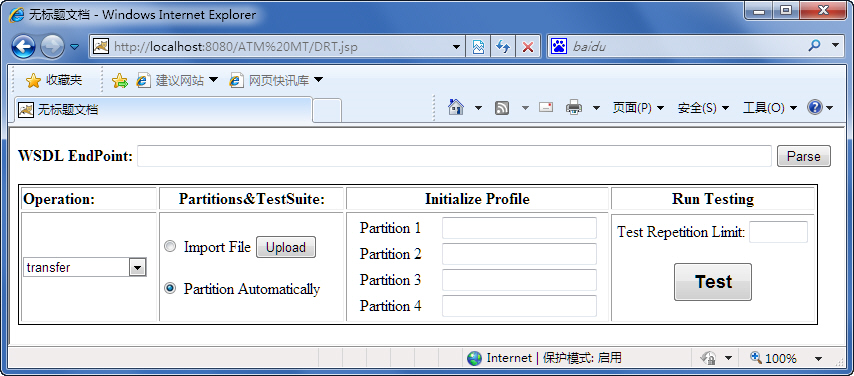
\includegraphics[width=0.5\textwidth]{fig//prototype}
  \caption{The snapshot of the prototype interfaces}
  \label{fig:prototype}
\end{figure}

\section{Empirical Study}
\label{sec:empiricalstudy}

We have conducted a series of empirical studies to evaluate the performance of DRT.

\subsection{Research Questions}

In our experiments, we focus on the following three research questions:

\begin{description}
  \item [RQ1] How effective is DRT in detecting faults of web services?

  The fault-detection effectiveness is one key criterion to evaluate the performance of a testing technique. In this study, three common real-life web services are selected as subject programs, and mutation analysis is used to evaluate the effectiveness.

  \item [RQ2] How does the number of partitions and the parameter of DRT affect the failure detection efficiency of DRT?

  In our earlier work~\cite{sun2012towards}, we found that the parameter of DRT have a significant effect on DRT efficiency, and the value of the parameter may be related to the number of partitions. The relationship between the parameter of DRT strategy and the number of partitions is obtained through theoretical analysis, which is verified through empirical studies.

  \item [RQ3] What is the actual test case generation overhead for DRT strategy.

  In Section~\ref{sec:DRTStrategy}, we have theoretically demonstrated that DRT only requires linear time for generating test case. We also wish to empirical evaluate the test case
generation and execution time required for detecting programs.
\end{description}

\subsection{Subject Web Services}

In our study, we selected three real-life web services, namely \texttt{Aviation Consignment Management Service\\ (ACMS)}, \texttt{China Unicom billing service (CUBS\\)}, \texttt{Parking billing service (PBS)}, as the subject programs of the experiments. Mutation analysis help us generate 1563 mutants for all objects. After identifying equivalent mutants, we only include those mutants being hard to detect for the evaluation. Further to say, every those mutants cannot be detected with less than 20 randomly generated test cases. Table~\ref{tab:objects} summarizes the basic information of the object web services. In following section, we give a detailed description of each web services.

\begin{table}[!htp]
\caption{Objects web services}
\label{tab:objects}
\centering
\begin{tabular}{|c|c|c|} \hline
  Web Services           &LOC           &Number of mutants \\ \hline
  ACMS    &116           &3   \\ \hline
  CUBS       &131           &11   \\ \hline
  PBS            &129           &4    \\ \hline
\end{tabular}

\end{table}

\subsubsection{Aviation Consignment Management Service (ACMC)}

The ACMS helps airline counter check the weight of free luggage and the cost of Overweight luggage. According to destinations, flights are divided into international and domestic flights. Each aircraft offers three kinds of cabins for passengers to choose: economy, business and first class. Passengers in different classes can enjoy different weight of luggage for free. The detailed billing rules are summarized in Table~\ref{tab:aviation}, where $price_0$ means economy class fare. When the flight is international, the weight of free luggage is different according to whether the passenger is a student or not. If the passenger is a student, the weight of luggage is 30kg, and 20kg otherwise.

\begin{table*}[!htp]
  \caption{The detailed billing rules of ACMC}
  \label{tab:aviation}
  \centering
  \begin{tabular}{|c|c|c|c|c|c|c|} \hline
  \multirow{2}{*}{}     &\multicolumn{3}{c|}{Domestic Flights}              &\multicolumn{3}{c|}{International Flights} \\
  \cline{2-7}
                       &first class  &business class   &economy class   &first class  &business class   &economy class \\ \hline
  hand carry~(kg)   &5       &5        &5        &7        &7        &7  \\ \hline
  checked-in for free~(kg)   &40      &30       &20       &40       &30       &20/30 \\ \hline
  Overweight billing~(kg)   &\multicolumn{3}{c|}{$price_0 * 1.5\%$}   &\multicolumn{3}{c|}{$price_0 * 1.5\%$}  \\ \hline
  \end{tabular}
\end{table*}

\subsubsection{China Unicom Billing Service (CUBS)}

CUBS provides an interface in which customers can know how much fee needed to pay according to cell-phone plans, cell-phone calls, and date usage. The details of various cell-phone plans are summarized in Tables~\ref{table:chinaA},~\ref{table:chinaB}, and~\ref{table:chinaC}.

% cell-phone plan~(CNY)
%\begin{table*}[!htp]
%  \caption{Cell-phone plan A}
%  \label{table:chinaA}
%  \centering
%  \begin{tabular}{|c|c|c|c|c|c|c|c|c|c|c|c|c|} \hline
%  \multicolumn{2}{|c|}{\mulitirow{2}{*}{}}                 &46  &66  &96  &126  &156  &186  &226  &286  &386  &586  &886 \\ \hline
%  \rule{0pt}{8pt}\multirow{3}{*}{\rotatebox{90}{contains}} &free calls~(min)  &50  &50  &240  &320  &420  &510  &700 &900 &1250 &1950  &3000 \\ \cline{2-13}
%  \rule{0pt}{8pt}                                          &free data~(MB)  &150 &300 &300  &400  &500  &650  &750 &950 &1300 &2000  &3000 \\ \cline{2-13}
%  \rule{0pt}{8pt}                                          &free incoming calls  &\multicolumn{11}{c|}{domestic~(including video calls)} \\ \hline
%  \rule{0pt}{8pt}\multirow{3}{*}{\rotatebox{90}{overuse}} &incoming calls~(CNY/min)  &0.25 &0.20  &\multicolumn{9}{c|}{0.15} \\ \cline{2-13}
%  \rule{0pt}{8pt}                                          &data~(CNY/KB)  &\multicolumn{11}{c|}{0.0003} \\ \cline{2-13}
%  \rule{0pt}{8pt}                                          &video calls~(CNY/min)  &\multicolumn{11}{c|}{0.60} \\ \hline
%  \end{tabular}
%\end{table*}




\begin{table*}[!htp]
  \caption{Cell-phone plan A}
  \label{table:chinaA}
  \centering
  \begin{tabular}{|c|c|c|c|c|c|c|c|c|c|c|c|c|} \hline
  \multicolumn{2}{|c|}{\multirow{2}{*}{plan's details}}                 &\multicolumn{11}{|c|}{cell-phone plan} \\ \cline{3-13}
  \multicolumn{2}{|c|}{}                                                        &$plan_1$  &$plan_2$  &$plan_3$  &$plan_4$  &$plan_5$  &$plan_6$ &$plan_7$  &$plan_8$  &$plan_9$  &$plan_{10}$  &$plan_{11}$ \\ \hline
  \rule{0pt}{8pt}\multirow{3}{*}{\rotatebox{90}{contains}} &free calls~(min)  &50  &50  &240  &320  &420  &510  &700 &900 &1250 &1950  &3000 \\ \cline{2-13}
  \rule{0pt}{8pt}                                          &free data~(MB)  &150 &300 &300  &400  &500  &650  &750 &950 &1300 &2000  &3000 \\ \cline{2-13}
  \rule{0pt}{8pt}                                          &free incoming calls  &\multicolumn{11}{c|}{domestic~(including video calls)} \\ \hline
  \rule{0pt}{8pt}\multirow{3}{*}{\rotatebox{90}{overuse}} &incoming calls~(CNY/min)  &0.25 &0.20  &\multicolumn{9}{c|}{0.15} \\ \cline{2-13}
  \rule{0pt}{8pt}                                          &data~(CNY/KB)  &\multicolumn{11}{c|}{0.0003} \\ \cline{2-13}
  \rule{0pt}{8pt}                                          &video calls~(CNY/min)  &\multicolumn{11}{c|}{0.60} \\ \hline
  \end{tabular}
\end{table*}

\begin{table}[!htp]
  \caption{Cell-phone plan B}
  \label{table:chinaB}
  \centering
\setlength{\tabcolsep}{1mm}{
  \begin{tabular}{|c|c|c|c|c|c|c|c|} \hline
    \multicolumn{2}{|c|}{\multirow{2}{*}{plan's details}}   &\multicolumn{6}{|c|}{cell-phone plan} \\ \cline{3-8}
    \multicolumn{2}{|c|}{}                                  &$plan_1$  &$plan_2$  &$plan_3$  &$plan_4$  &$plan_5$  &$plan_6$   \\ \hline
    \rule{0pt}{8pt}\multirow{3}{*}{\rotatebox{90}{contains}} &free calls~(min)  &120  &200  &450  &680  &920  &1180 \\ \cline{2-8}
    \rule{0pt}{8pt}                                          &free data~(MB)  &40 &60 &80  &100  &120  &150 \\ \cline{2-8}
    \rule{0pt}{8pt}                                          &free incoming calls  &\multicolumn{6}{c|}{domestic(including video calls)} \\ \hline
    \rule{0pt}{8pt}\multirow{3}{*}{\rotatebox{90}{overuse}} &incoming calls~(CNY/min)  &0.25 &0.20  &\multicolumn{4}{c|}{0.15} \\ \cline{2-8}
    \rule{0pt}{8pt}                                          &data~(CNY/KB)  &\multicolumn{6}{c|}{0.0003} \\ \cline{2-8}
    \rule{0pt}{8pt}                                          &video calls~(CNY/min)  &\multicolumn{6}{c|}{0.60} \\ \hline
  \end{tabular}}
\end{table}

\begin{table}[!htp]
  \caption{Cell-phone plan C}
  \label{table:chinaC}
  \centering
  \begin{tabular}{|c|c|c|c|c|} \hline
  \multicolumn{2}{|c|}{\multirow{2}{*}{plan's details}}  &\multicolumn{3}{|c|}{cell-phone plan~(CNY)} \\ \cline{3-5}
  \multicolumn{2}{|c|}{}                                  &$plan_1$  &$plan_2$  &$plan_3$ \\ \hline
  \rule{0pt}{8pt} \multirow{3}{*}{\rotatebox{90}{contains}} &free calls~(min)  &260  &380  &550 \\ \cline{2-5}
  \rule{0pt}{8pt}                                          &free data~(MB)  &40 &60 &80 \\ \cline{2-5}
  \rule{0pt}{8pt}                                          &free data~(MB)  &\multicolumn{3}{c|}{domestic~(including video calls)} \\ \hline
  \rule{0pt}{8pt} \multirow{3}{*}{\rotatebox{90}{overuse}} &incoming calls~(CNY/min)  &0.25 &0.20  &0.15 \\ \cline{2-5}
  \rule{0pt}{8pt}                                          &data~(CNY/KB)  &\multicolumn{3}{c|}{0.0003} \\ \cline{2-5}
   \rule{0pt}{8pt}                                         &video calls~(CNY/min)  &\multicolumn{3}{c|}{0.60} \\ \hline
  \end{tabular}
\end{table}


%\begin{table}[!htp]
%  \caption{Cell-phone plan C}
%  \label{table:chinaC}
%  \centering
%  \begin{tabular}{|c|c|c|c|c|} \hline
%  \multicolumn{2}{|c|}{cell-phone plan~(CNY)}  &46  &66  &96   \\ \hline
%  \rule{0pt}{8pt} \multirow{3}{*}{\rotatebox{90}{contains}} &free calls~(min)  &260  &380  &550 \\ \cline{2-5}
%  \rule{0pt}{8pt}                                          &free data~(MB)  &40 &60 &80 \\ \cline{2-5}
%  \rule{0pt}{8pt}                                          &free data~(MB)  &\multicolumn{3}{c|}{domestic~(including video calls)} \\ \hline
%  \rule{0pt}{8pt} \multirow{3}{*}{\rotatebox{90}{overuse}} &incoming calls~(CNY/min)  &0.25 &0.20  &0.15 \\ \cline{2-5}
%  \rule{0pt}{8pt}                                          &data~(CNY/KB)  &\multicolumn{3}{c|}{0.0003} \\ \cline{2-5}
%   \rule{0pt}{8pt}                                         &video calls~(CNY/min)  &\multicolumn{3}{c|}{0.60} \\ \hline
%  \end{tabular}
%\end{table}

\subsubsection{Parking Billing Service (PBS)}

Consider a parking billing service, which accepts the parking details of each vehicle, including type of vehicle, day of week, discount coupon, and hours of parking. This service first rounds up the parking duration to the next full hour, and than calculates the parking fee for a vehicle according to the hourly rates in Table~\ref{tab:hourlyRate}. If a voucher discount is presented, a 50\% discount off the parking fee will be given.

\begin{table*} [!htp]\small
  \caption{Hourly parking rates}
  \label{tab:hourlyRate}
  \centering
  \begin{tabular}{|c|c|c|c|c|c|c|} \hline
  \multirow{3}{*}{Actual parking hours}                        &\multicolumn{6}{|c|}{Hourly parking rates} \\ \cline{2-7}
                                   &\multicolumn{3}{|c|}{Weekday}     &\multicolumn{3}{|c|}{Saturday and Sunday} \\ \cline{2-7}
                                  &Motorcycle  &Car:2-door coupe  &Car:others    &Motorcycle  &Car:2-door coupe  &Car:others \\ \hline
  $(0.0,2.0]$                     &4.00\$        &4.50\$          &5.00\$      &5.00\$        &6.00\$        &7.00\$ \\ \hline
  $(2.0,4.0]$                     &5.00\$        &5.50\$          &6.00\$      &6.50\$      &7.50\$        &8.50\$  \\ \hline
  $(4.0,24.0]$                    &6.00\$        &6.50\$          &7.00\$      &8.00\$      &9.00\$        &10.00\$  \\ \hline
  \end{tabular}
\end{table*}

To facilitate better parking management, at the time of parking, customers can optionally provide an estimation of parking duration in terms of three different time ranges, namely $(0.0,2.0]$, $(2.0,4.0]$, and $(4.0,24.0]$. Suppose a customer providers an estimation. If the estimated hours of parking and the actual hours of parking fall into the same time range, then the customer will receive a 40\% discount. If the estimated hours and the actual hours are in different time range, a 20\% markup will be added. A customer may also choose to either use a discount coupon, or provide an estimation of parking duration, but not both. Obviously, a customer may also choose to neither provide an estimation, nor use a discount coupon. Note that no vehicles are allowed to park across two consecutive days on a continuous basis.

\subsection{Variables}

\subsubsection{Independent Variables}

The independent variable in our study is the testing technique. The DRT technique must be chosen for this variable. In addition, we selected RPT and RT as the baseline techniques for comparison.

\subsubsection{Dependent Variables}

The dependent variable for RQ1 is the metric for evaluating the fault-detection effectiveness. There exist quite a few effectiveness metrics, such as the P-measure (the probability of at least one fault being detected by a test suite), the E-measure (the expected number of faults being detected by a test suite), the F-measure (the expected number of test cases to detect the first fault), and the T-measure (the expected number of test cases to detect all faults). Among them, the F-measure and T-measure are the most appropriate metrics for measuring the fault-detection effectiveness of DRT testing techniques. In our study, we use $F$, $T$ to represent the F-measure and the T-measure of a testing method. and $SD_{measure}$ represents the standard deviation of
As shown in Algorithm~\ref{alg:DRT}, the testing process may not be terminated after the detection of the first fault. In addition, the fault detection information can lead to different probability profile adjustment mechanisms. Therefore, it is also important to see what would happen after the first fault is revealed. In our study, we introduce a new metric F2-measure, which refers to how many additional test cases are required to reveal the second fault after the detection of the first fault. Similarly, we use $F2$ to represent the F2-measure of a testing method, and $SD_{measure}$ represents standard deviation of metrics, where $measure$ can be F, F2, and T.

For RQ3, an obvious metric is the time required on detecting faults. In this study, corresponding to the T-measure, we used the $T$-$time$ to measure the time for detecting all faults, respectively. Similarly, $F$-$time$ and $F2$-$time$ are used to denote the time required for detecting the first and the additional time for detecting the second faults after detecting the first fault, respectively.

For each of the above four metrics, a smaller value intuitively implies a better performance.

\subsection{Experimental Settings}

\subsubsection{Partitioning}

In our study, we made use of the decision table~\cite{gettys1986if, tao2017entropy}, a typical PT technique, to conduct the partitions. A decision table is based on a simple principle: sets of actions for sets of constrains. It is used to present a large quantity of complex information in a simple, straightforward manner. Usually, a decision table is composed of the constraint part and action part. Constraints are the pre-conditions of a contract and have to be resolvable to true or false. The action part specifies valid system responses with respect to constrains, called \emph{rules}. The action part represents the post-conditions of a contract. Thus, every rule of the decision table defines a \emph{contract}. In our study, every \emph{contract} corresponds to a partition.

To investigate the performance of three testing techniques under various scenarios, we develop two partition schemas shown in Table~\ref{tab:partition}:

\begin{itemize}
\item \textbf{Scheme 1}: every \emph{contract} in the decision table corresponds to a partition.
\item \textbf{Scheme 2}: After constructing the decision table, we group those contraints with the same responses, then every \emph{contract} in the decision table corresponds to a partition.
\end{itemize}

\begin{table}[!htbp]
\caption{Two partition schemas}
\label{tab:partition}
\centering
\begin{tabular}{|c|c|c|} \hline
  web services      &Scheme 1         &Scheme 2  \\ \hline
  ACMS  &24                &7          \\ \hline
  CUBS      &20                &3          \\ \hline
  PBS      &18                &3          \\ \hline

\end{tabular}
\end{table}

\subsubsection{Initial Test Profile}

Since the test cases are randomly generated during the test process, it is a conservative and feasible method to use the equal probability distribution as the initial testing profile. On the other hand, testers can also apply past experience to use a unequal probability distribution as the initial testing profile.

\subsubsection{Constants}

In the experiments,  we explore the relationship between the number of partitions and parameter of DRT strategy. Therefore, we design a set of parameter values, $\varepsilon \in \{1.0E$-$05, 5.0E$-$05, 1.0E$-$04, 5.0E$-$04, 1.0E$-$03, 5.0E$-$03, 1.0E$-$02, 5.0E$-$02, 1.0E$-$01, 2E$-$01, 3E$-$01, 4E$-$01, 5E$-$01\}$. Note that $\varepsilon = 5E$-$01$ is already a big one. Consider this Scenario:
In PBS, when the test is carried out under the partition scheme 2, if we set $\varepsilon = 7.5E$-$01$ and equal probability distribution as testing profile, that is, $p_i = 1/3$. Suppose that the first test case belongs to $c_1$ was executed and did not reveal any faults, then the value of $p_1$ would be 0 according to Formula 3. Thus, the value of $\varepsilon$ should not be too big.

\subsection{Experimental Environment}

Our experiments were conducted on a virtual machine running the Ubuntu 11.06 64-bit operating system. In this system, there were two CPUs and a memory of 2GB. The test scripts were generated using Java. In the experiments, we repeatedly run the testing using each technique for 30 times with 30 seeds to guarantee the statistically reliable mean values of the metrics (F-measure, F2-measure, T-measure, F-time, F2-time, T-time).


\subsection{Threats To Validity}

\subsubsection{Internal Validity}

The threat to internal validity is related to the implementations of the testing techniques, which involved a moderate amount of programming work. The code was also cross-checked by different individuals. We are confident that all techniques were correctly implemented.

\subsubsection{External Validity}

One obvious threat to external validity is that we only considered three object web services. However, they are real-life web services. In addition, 17 distinct faults were used to evaluate the performance. Though we have tried to improve the generality by applying different granularities in partitioning and 13 kinds of parameters, we cannot say whether or not similar results would be observed in other types of web services.

\subsubsection{Construct Validity}

The metrics used in our study are simple in concept and straightforward to apply, hence the threat to construct validity is little.

\subsubsection{Conclusion Validity}

We have run a sufficient number of trials to guarantee the statistical reliability of our experimental results. In addition, as to be discussed in Section~\ref{sec:results}, statistical tests were conducted to verify the significance of our results.

\begin{table*}
  \caption{The results of ACMS}
  \label{result:aviation}
  \centering
  \begin{tabular}{|c|c|c|c|c|c|c|c|c|c|c|c|c|c|} \hline
     \multicolumn{2}{|c|}{\multirow{2}{*}{Strategy}} &\multicolumn{6}{|c|}{Partition Schema 1} &\multicolumn{6}{|c|}{Partition Schema 2}\\ \cline{3-14}
     \multicolumn{2}{|c|}{}  &F       &$SD_F$  &F2    &$SD_{F2}$  &T     &$SD_T$  &F     &$SD_F$  &F2    &$SD_{F2}$  &T     &$SD_T$  \\ \hline
     \multicolumn{2}{|c|}{RT}  &13.30   &10.34   &14.90 &24.64      &41.80 &27.13   &13.30 &10.34   &14.90 &24.64      &41.80 &27.13   \\ \hline
     \multicolumn{2}{|c|}{RPT} &12.04   &11.13   &12.26 &19.08      &35.31 &25.95   &9.03  &8.24    &15.13 &16.08      &34.29 &29.53   \\ \hline
     \multirow{13}{*}{DRT} &1.0E-5  &11.42  &10.16  &11.93  &18.62  &34.93  &22.46  &8.73   &9.88   &13.28  &18.83  &36.19  &28.96  \\ \cline{2-14}
                           &5.0E-5	&12.42	&10.63	&12.05	&20.27	&36.90	&25.39	&8.65	&9.30	&13.53	&19.07	&35.76	&29.86 \\ \cline{2-14}
                           &1.0E-4	&11.34	&10.65	&11.66	&21.27	&35.19	&26.01	&7.36	&8.49	&13.09	&17.89	&33.00	&27.94 \\ \cline{2-14}
                           &5.0E-4	&12.16	&12.13	&11.50	&19.36	&34.19	&26.18	&7.80	&8.37	&13.45	&17.36	&33.59	&27.67 \\ \cline{2-14}
                           &1.0E-3	&11.46	&11.10	&11.39	&19.01	&34.86	&23.17	&7.68	&8.11	&15.07	&19.85	&33.65	&29.95 \\ \cline{2-14}
                           &5.0E-3	&11.02	&9.67	&12.24	&18.83	&32.92	&20.75	&7.47	&8.65	&15.40	&18.81	&35.14	&29.01 \\ \cline{2-14}
                           &1.0E-2	&10.48	&9.60	&9.46	&14.17	&29.59	&19.10	&7.66	&9.18	&14.93	&18.69	&34.30	&30.15 \\ \cline{2-14}
                           &5.0E-2	&8.75	&6.59	&7.06	&10.35	&23.05	&11.67	&7.26	&7.74	&14.70	&18.15	&34.81	&28.14 \\ \cline{2-14}
                           &1.0E-1	&8.59	&6.66	&6.37	&9.41	&21.36	&10.81	&6.67	&7.34	&16.26	&17.54	&34.27	&27.48 \\ \cline{2-14}
                           &2.0E-1	&8.50	&6.21	&5.80	&9.07	&22.10	&10.56	&5.71	&6.04	&16.63	&10.33	&33.58	&30.78 \\ \cline{2-14}
                           &3.0E-1	&9.23	&6.84	&7.12	&10.34	&22.57	&11.13	&5.43	&6.28	&17.60	&10.39	&33.86	&30.33 \\ \cline{2-14}
                           &4.0E-1	&9.22	&7.03	&6.72	&9.36	&22.57	&10.44	&5.14	&5.19	&17.56	&19.11	&33.83	&28.94 \\ \cline{2-14}
                           &5.0E-1	&8.61	&6.41	&7.70	&10.45	&22.64	&10.95	&5.86	&6.50	&16.18	&17.06	&33.31	&27.40 \\ \hline
  \end{tabular}
\end{table*}

\begin{table*}
  \caption{The results of CUBS}
  \label{result:china}
  \centering
  \begin{tabular}{|c|c|c|c|c|c|c|c|c|c|c|c|c|c|} \hline
     \multicolumn{2}{|c|}{\multirow{2}{*}{Strategy}} &\multicolumn{6}{|c|}{Partition Schema 1} &\multicolumn{6}{|c|}{Partition Schema 2}\\ \cline{3-14}
     \multicolumn{2}{|c|}{}  &F       &$SD_F$  &F2    &$SD_{F2}$  &T     &$SD_T$  &F     &$SD_F$  &F2    &$SD_{F2}$  &T     &$SD_T$  \\ \hline
     \multicolumn{2}{|c|}{RT}  &21.93	&20.37	&38.17	&38.17	&4203.07	&3219.40	&21.93	&20.37	&38.17	&38.17	&4203.07	&3219.40	\\ \hline
     \multicolumn{2}{|c|}{RPT} &21.96	&20.36	&28.74	&27.56	&2590.38	&1768.49	&23.66	&21.92	&27.31	&26.99	&4195.72	&2777.89	\\ \hline
     \multirow{13}{*}{DRT} &1.0E-5	&21.21	&23.24	&25.62	&23.29	&2720.70	&2051.85	&22.90	&22.51	&25.29	&28.21	&4106.81	&2589.29	\\ \cline{2-14}
                           &5.0E-5	&19.50	&19.94	&25.77	&24.78	&2503.45	&1873.76	&23.88	&23.25	&26.68	&26.84	&4130.03	&2588.36	\\ \cline{2-14}
                           &1.0E-4	&20.71	&22.51	&25.59	&26.00	&2516.91	&1843.11	&23.55	&22.76	&26.71	&30.26	&4196.01	&2247.57	\\ \cline{2-14}
                           &5.0E-4	&21.79	&21.10	&26.82	&28.21	&2519.39	&1942.65	&25.27	&28.74	&26.11	&24.36	&4190.61	&2753.74	\\ \cline{2-14}
                           &1.0E-3	&20.95	&20.79	&31.41	&31.54	&2532.84	&1752.56	&23.84	&25.44	&27.34	&27.64	&4291.41	&2884.39	\\ \cline{2-14}
                           &5.0E-3	&22.32	&21.90	&25.93	&26.48	&2535.97	&1572.42	&24.11	&23.27	&26.80	&25.20	&4218.74	&2887.01	\\ \cline{2-14}
                           &1.0E-2	&22.47	&21.55	&26.01	&23.85	&2550.88	&1873.01	&23.46	&25.01	&26.74	&26.43	&4117.11	&2798.92	\\ \cline{2-14}
                           &5.0E-2	&21.61	&20.04	&27.66	&29.12	&2559.56	&1777.16	&24.01	&24.32	&26.52	&27.04	&4105.51	&2570.57	\\ \cline{2-14}
                           &1.0E-1	&21.72	&21.71	&28.31	&28.91	&2533.08	&1774.39	&23.30	&24.45	&26.07	&27.91	&4271.32	&3011.37	\\ \cline{2-14}
                           &2.0E-1	&21.71	&21.83	&28.68	&32.75	&2552.29	&1879.60	&23.55	&25.20	&28.25	&30.31	&4170.32	&2796.61	\\ \cline{2-14}
                           &3.0E-1	&22.82	&21.65	&26.68	&31.28	&2623.00	&1770.36	&23.40	&25.52	&27.35	&27.84	&4138.49	&2594.70	\\ \cline{2-14}
                           &4.0E-1	&23.34	&24.02	&27.32	&27.42	&2664.34	&1886.21	&23.07	&24.08	&29.18	&30.39	&4192.68	&2706.73	\\ \cline{2-14}
                           &5.0E-1	&22.18	&22.32	&27.14	&28.54	&2599.40	&1640.05	&23.30	&23.63	&26.98	&27.71	&4195.45	&2535.00	\\ \hline
  \end{tabular}
\end{table*}

\begin{table*}
  \caption{The results of PBS}
  \label{result:parking}
  \centering
  \begin{tabular}{|c|c|c|c|c|c|c|c|c|c|c|c|c|c|} \hline
     \multicolumn{2}{|c|}{\multirow{2}{*}{Strategy}} &\multicolumn{6}{|c|}{Partition Schema 1} &\multicolumn{6}{|c|}{Partition Schema 2}\\ \cline{3-14}
     \multicolumn{2}{|c|}{}   &F       &$SD_F$  &F2    &$SD_{F2}$  &T     &$SD_T$  &F     &$SD_F$  &F2    &$SD_{F2}$  &T     &$SD_T$  \\ \hline
     \multicolumn{2}{|c|}{RT}  &20.17   &16.32   &16.50 &13.20      &252.80 &191.54   &20.17   &16.32   &16.50 &13.20      &252.80 &191.54   \\ \hline
     \multicolumn{2}{|c|}{RPT} &17.71   &16.78   &16.72 &25.12      &178.91 &147.96   &16.49  &15.76    &15.45 &21.76      &182.66 &130.43  \\ \hline
     \multirow{13}{*}{DRT} &1.0E-5	&18.07	&19.08	&14.27	&21.70	&176.18	&146.49	&15.24	&15.06	&15.31	&23.97	&163.51	&135.48	\\ \cline{2-14}
                           &5.0E-5	&18.23	&18.34	&15.39	&24.35	&176.93	&143.93	&15.13	&15.35	&14.30	&23.57	&160.82	&116.59	\\ \cline{2-14}
                           &1.0E-4	&16.39	&17.42	&13.96	&21.04	&171.61	&142.79	&15.14	&15.05	&13.96	&22.31	&159.93	&121.90	\\ \cline{2-14}
                           &5.0E-4	&16.75	&17.56	&12.60	&21.98	&165.94	&140.33	&14.95	&12.66	&14.98	&24.52	&166.18	&125.20	\\ \cline{2-14}
                           &1.0E-3	&17.96	&18.93	&15.40	&22.22	&164.56	&138.74	&15.72	&16.03	&16.30	&24.41	&166.27	&128.63	\\ \cline{2-14}
                           &5.0E-3	&16.93	&17.23	&14.34	&22.34	&160.70	&117.02	&15.54	&12.79	&15.45	&23.70	&170.14	&129.61	\\ \cline{2-14}
                           &1.0E-2	&17.12	&16.60	&15.10	&22.68	&166.15	&136.59	&15.19	&15.02	&15.13	&25.78	&166.60	&124.97	\\ \cline{2-14}
                           &5.0E-2	&17.02	&18.70	&16.46	&24.75	&168.20	&129.72	&17.10	&17.23	&15.07	&24.09	&170.09	&130.88	\\ \cline{2-14}
                           &1.0E-1	&17.09	&16.78	&14.12	&22.00	&172.94	&153.50	&16.02	&17.16	&15.98	&24.97	&174.16	&134.34	\\ \cline{2-14}
                           &2.0E-1	&17.45	&18.36	&14.14	&22.77	&174.71	&139.02	&15.27	&15.54	&15.52	&23.86	&167.07	&132.81	\\ \cline{2-14}
                           &3.0E-1	&17.23	&18.45	&16.95	&27.43	&178.09	&161.44	&15.43	&15.54	&15.15	&22.04	&175.02	&136.66	\\ \cline{2-14}
                           &4.0E-1	&17.05	&17.72	&16.21	&20.08	&169.21	&145.43	&15.28	&15.93	&15.28	&24.48	&164.67	&124.24	\\ \cline{2-14}
                           &5.0E-1	&17.17	&18.26	&16.23	&25.83	&172.29	&134.94	&16.10	&15.78	&15.26	&23.80	&167.21	&124.05	\\ \hline
  \end{tabular}
\end{table*}




\section{Experimental Results}
\label{sec:results}

\subsection{RQ1: Fault Detection Effectiveness}
\label{sec:1}

The experimental results of F-measure, F2-measure and T-measure are summarized in Tables~\ref{result:aviation} to~\ref{result:parking}. The distributions of F-measure, F2-measure and T-measure on each object program are displayed by the boxplots in Figures~\ref{fig:Fmeasure} to~\ref{fig:Tmeasure}. In the boxplot, the upper and lower bounds of the box represent the third and first quartiles of a metric, respectively, and the middle line represent the median value. The upper and lower whiskers respectively indicate the largest and smallest data within the range of $\pm 1.5 \times IQR$, where $IQR$ is the interquartile range. The outliers outside $IQR$ are denoted by hollow circles. The solid circle represents the mean value of a metric.



\begin{figure*}
	\centering
    \subfigure[ACMS] {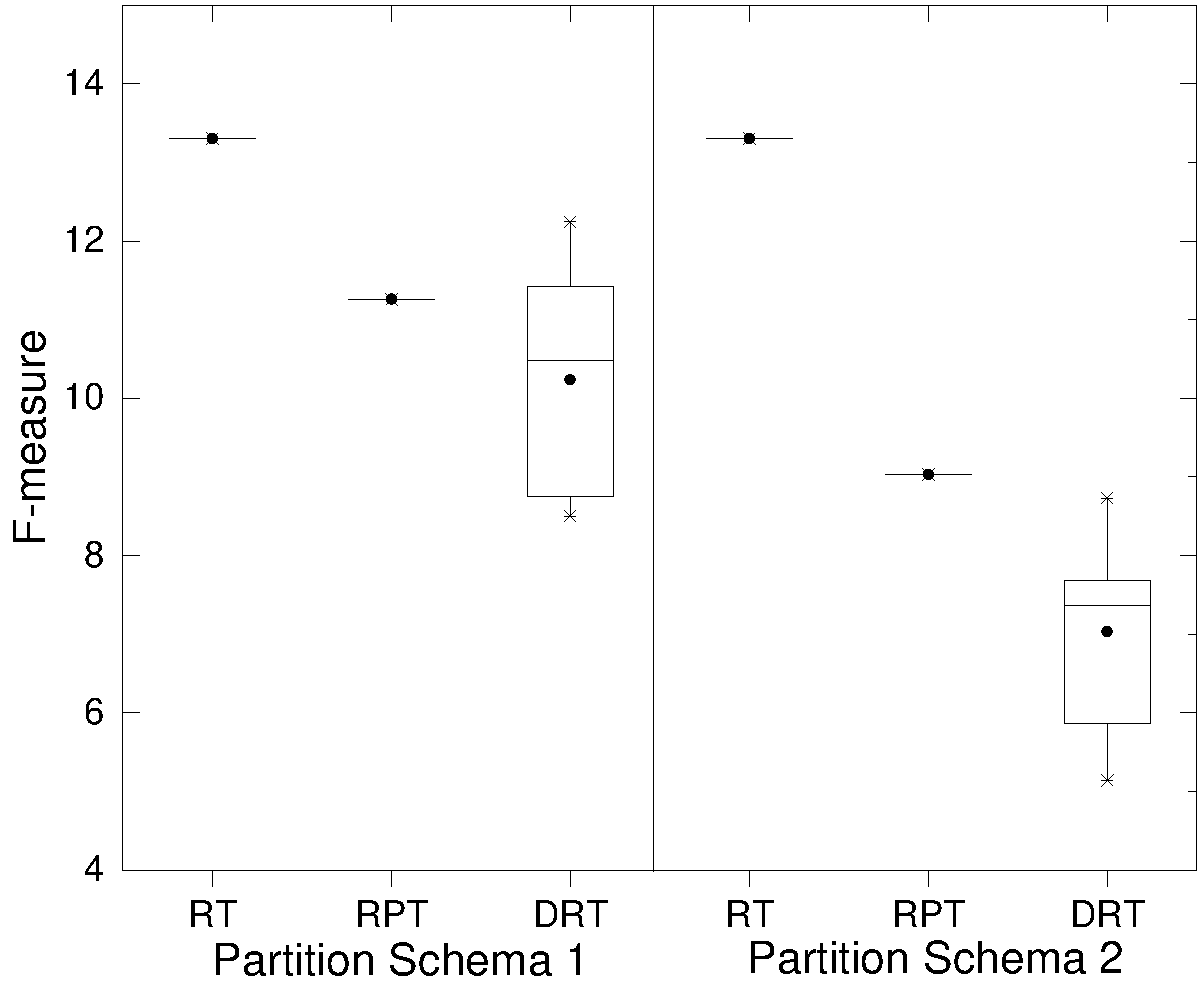
\includegraphics[width=0.32\textwidth,height=4cm]{fig/drtresultbox/aviaresultf.pdf}}
	\subfigure[CUBS] {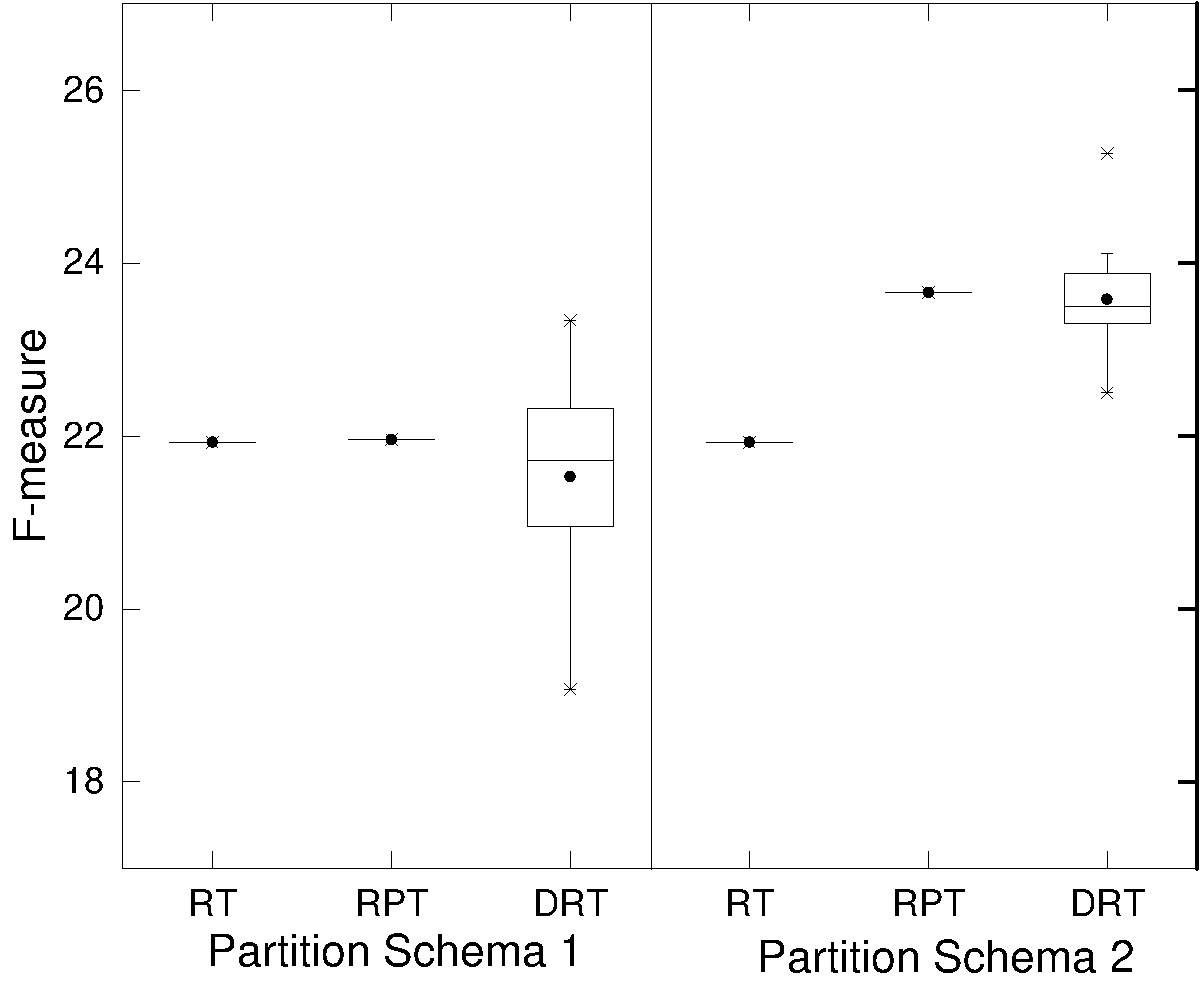
\includegraphics[width=0.32\textwidth,height=4cm]{fig/drtresultbox/chinaresultf.pdf}}
	\subfigure[PBS] {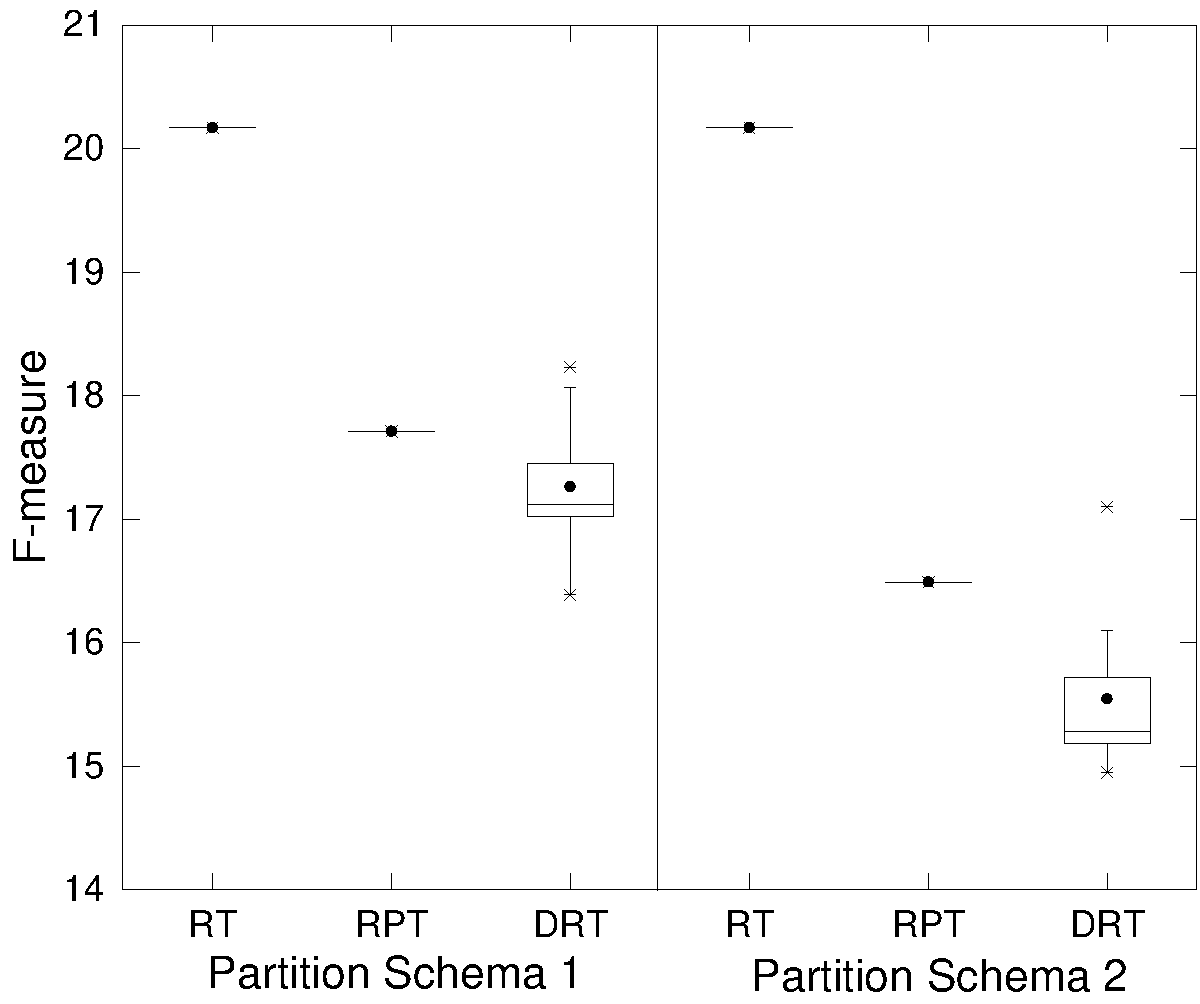
\includegraphics[width=0.32\textwidth,height=4cm]{fig/drtresultbox/parkingresultf.pdf}}
	\caption{Boxplots of F-measures on each object program}
	\label{fig:Fmeasure}
\end{figure*}

\begin{figure*}
	\centering
	\subfigure[ACMS] {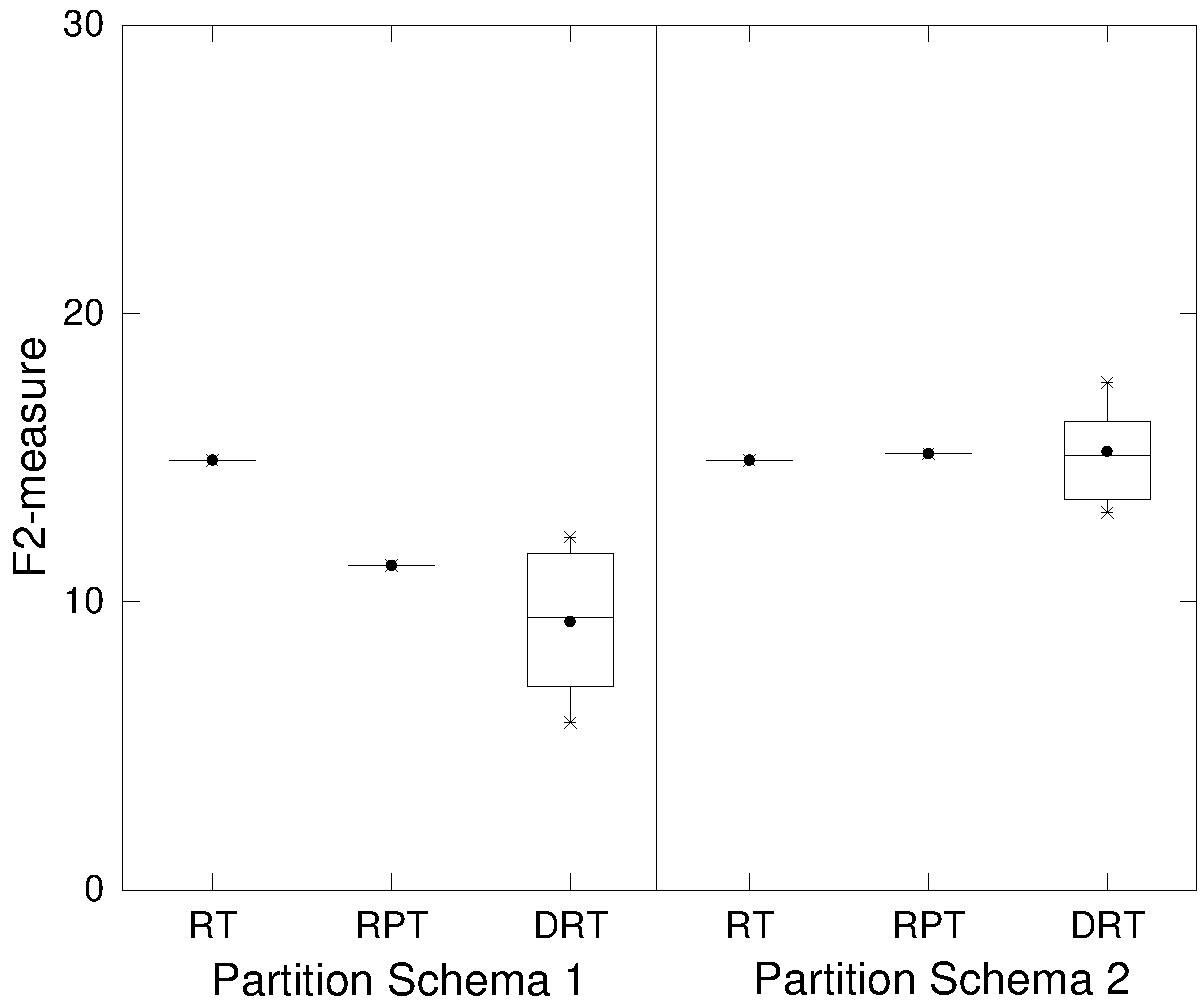
\includegraphics[width=0.32\textwidth,height=4cm]{fig/drtresultbox/aviaresultf2.pdf}}
	\subfigure[CUBS] {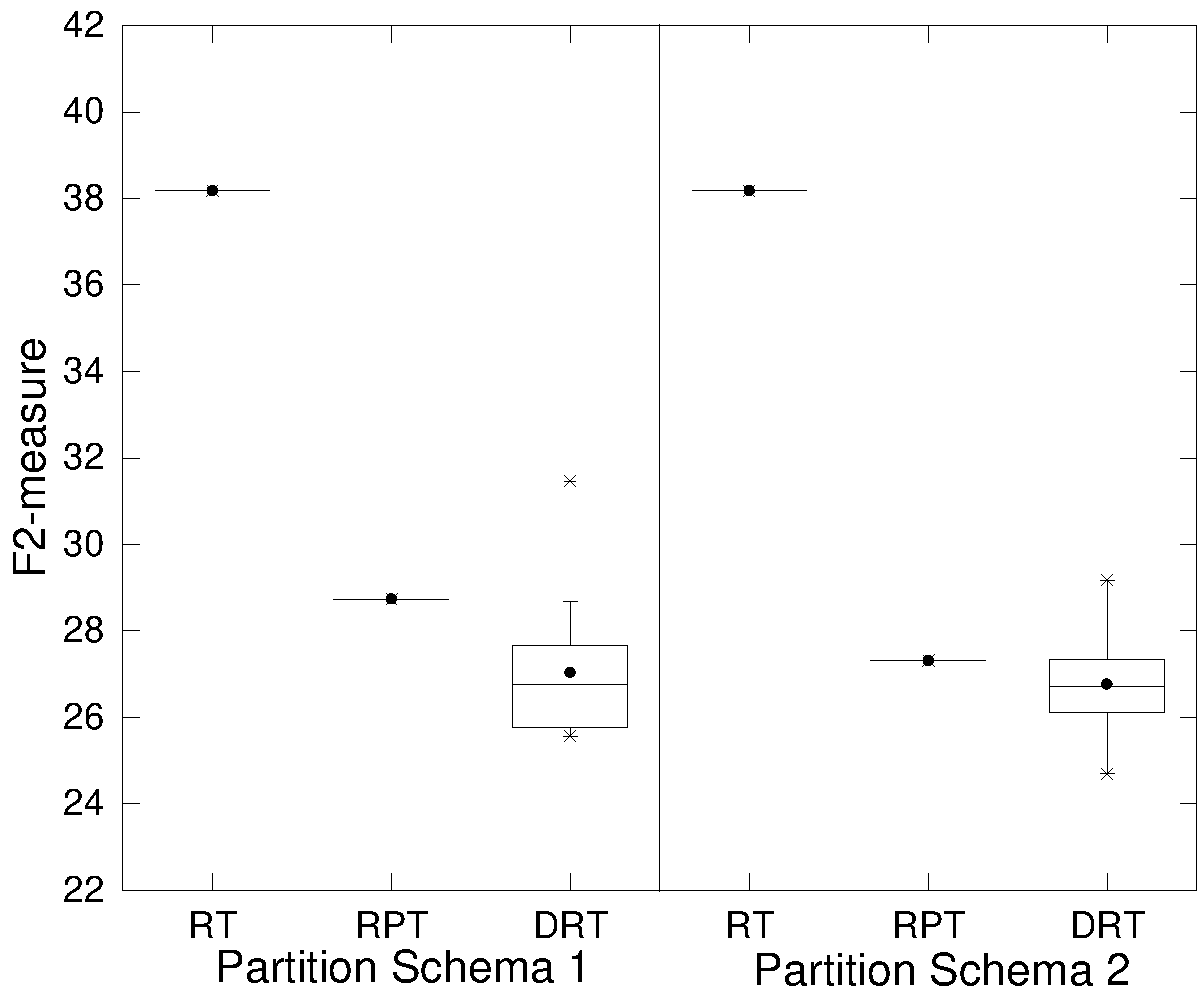
\includegraphics[width=0.32\textwidth,height=4cm]{fig/drtresultbox/chinaresultf2.pdf}}
	\subfigure[PBS] {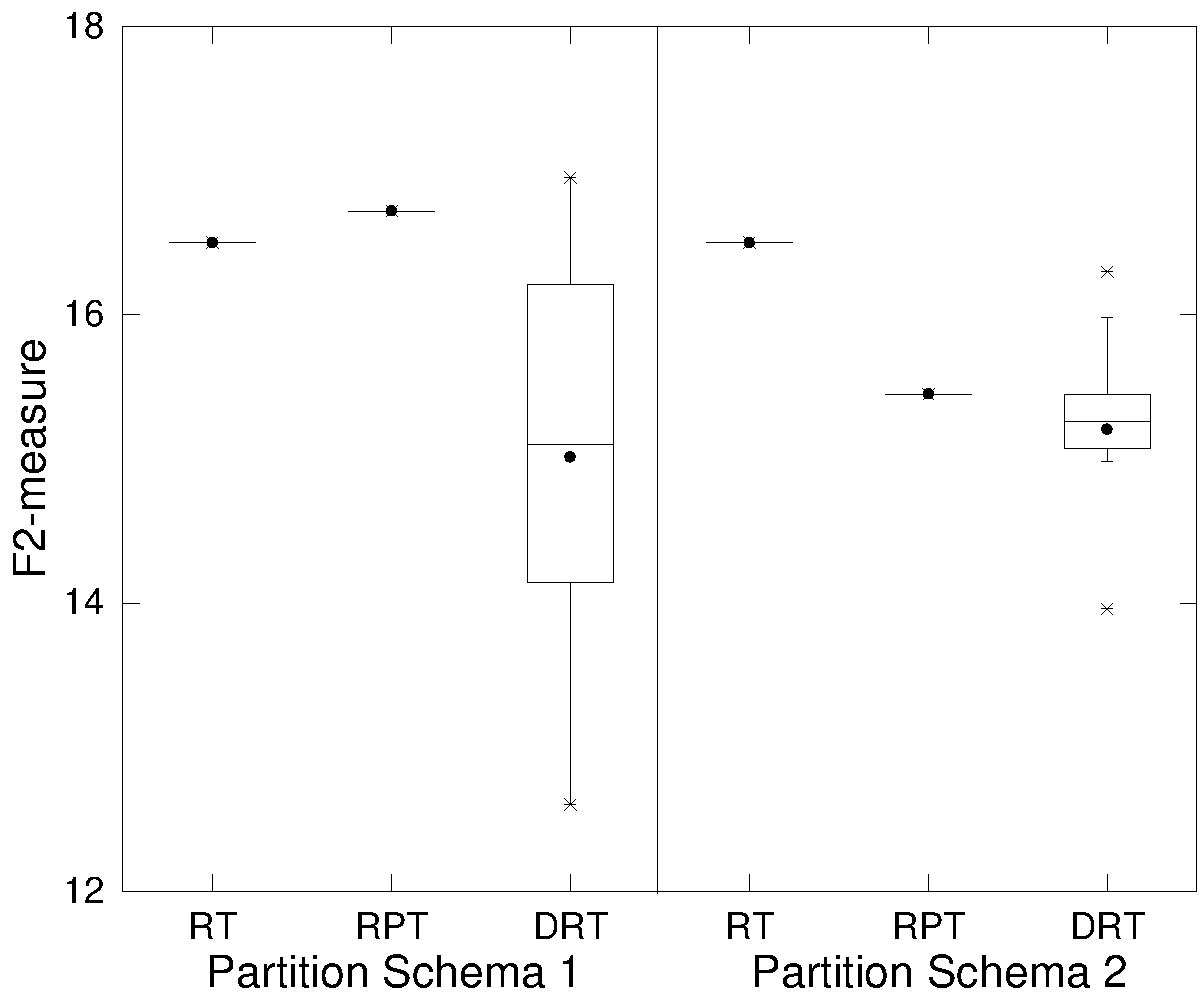
\includegraphics[width=0.32\textwidth,height=4cm]{fig/drtresultbox/parkingresultf2.pdf}}
	\caption{Boxplots of F2-measures on each object program}
	\label{fig:F2measure}
\end{figure*}

\begin{figure*}
	\centering
	\subfigure[ACMS] {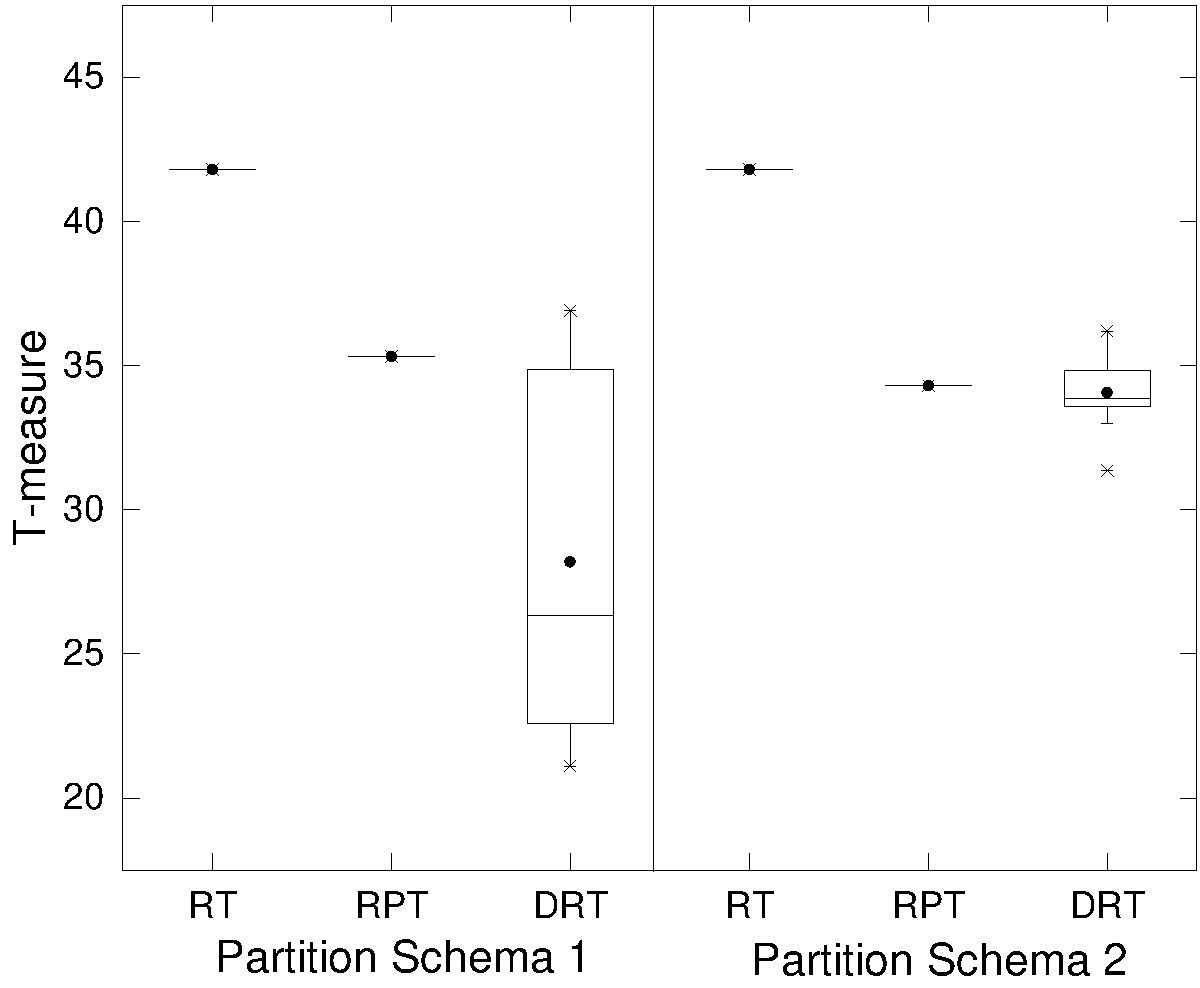
\includegraphics[width=0.32\textwidth,height=4cm]{fig/drtresultbox/aviaresultt.pdf}}
	\subfigure[CUBS] {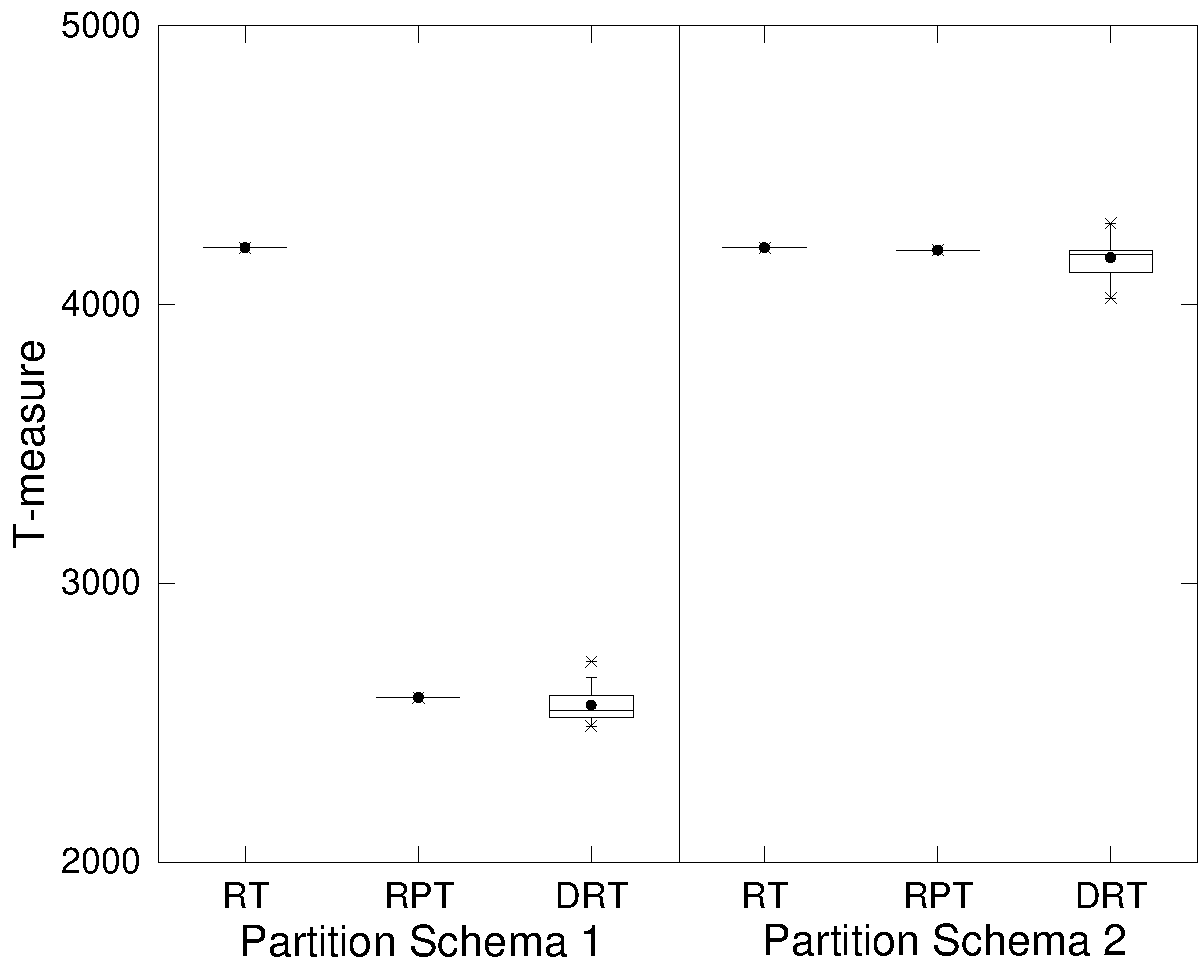
\includegraphics[width=0.32\textwidth,height=4cm]{fig/drtresultbox/chinaresultt.pdf}}
	\subfigure[PBS] {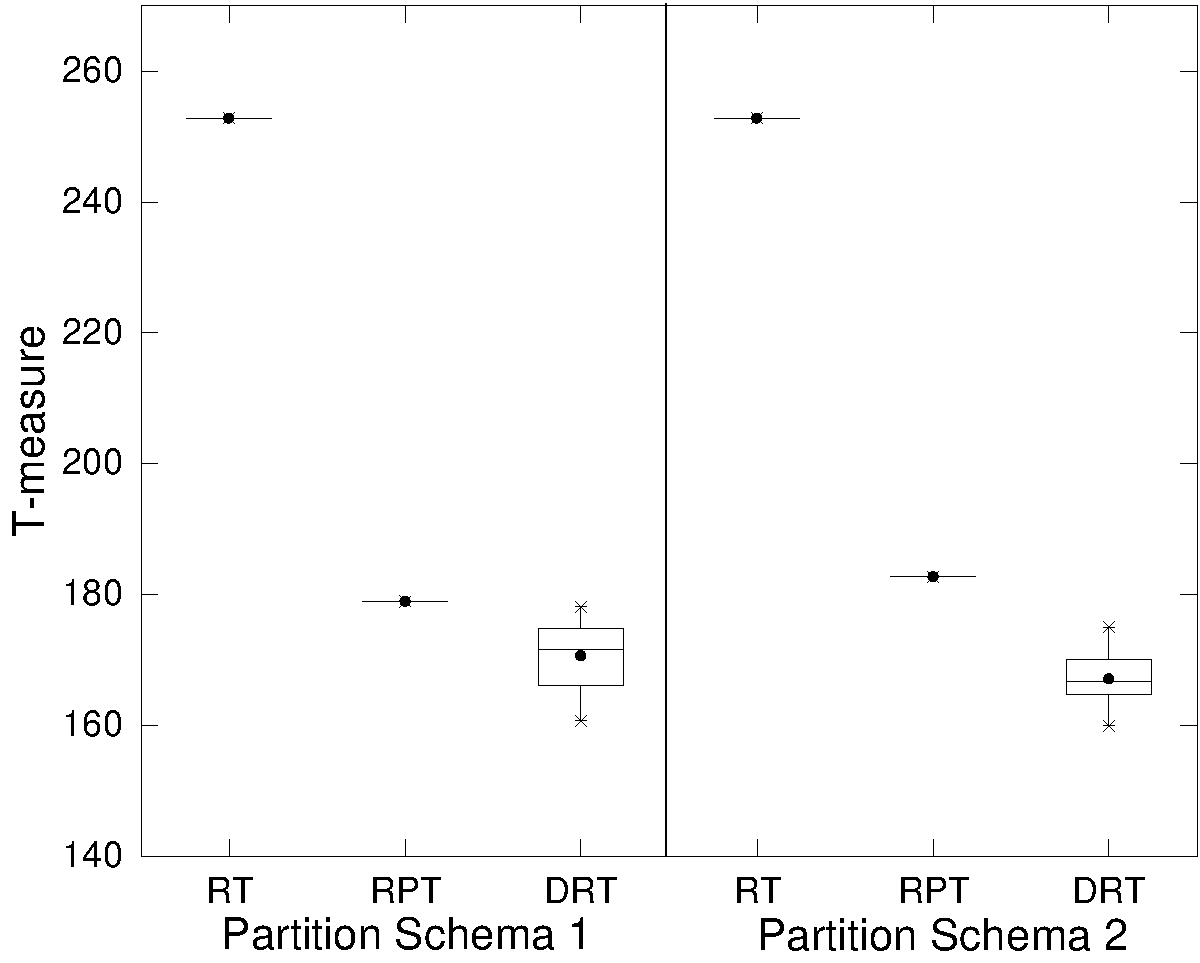
\includegraphics[width=0.32\textwidth,height=4cm]{fig/drtresultbox/parkingresultt.pdf}}
	\caption{Boxplots of T-measures on each object program}
	\label{fig:Tmeasure}
\end{figure*}

From Tables~\ref{result:aviation} to~\ref{result:parking} and Figures~\ref{fig:Fmeasure} to \ref{fig:Tmeasure}, we can observe that in general, DRT was the best performer in terms of F-measure, F2-measure, and T-measure, followed by RPT. We further conducted statistical testing to verify the significance of this observation. We used the Holm-Bonferroni method~\cite{Holm79} (with p-value being 0.05) to determine which pairs of testing techniques have significant difference. The statistical testing results are shown in Tables~\ref{tableHolm:fmeasure},~\ref{tableHlom:nfmeasure} and~\ref{tableHlom:tmeasure}. Each cell in the tables gives the number of scenarios where the technique on the top row performed better than that on the left column. If the difference is significant, the number will be displayed in bold. For example, the bold 76 in the top right corner in Table~\ref{tableHlom:nfmeasure} indicates that out of 78 scenarios (13 parameters $\times$ 2 partition schemas $\times$ 3 object web services), DRT had smaller F2-measure than RT for 69 scenarios, and the fault-detection capabilities of these two techniques were significantly different.
\begin{table}[htbp]
  \caption{Number of scenarios where the technique on top row has smaller F-measure than that on left column}
  \centering
  \label{tableHolm:fmeasure}
  \begin{tabular}{|c|c|c|c|} \hline
          &RT         &RPT         &DRT         \\ \hline
    RT    & ---       &\textbf{4}  &\textbf{60} \\ \hline
    RPT   &\textbf{2} & ---        &\textbf{61} \\ \hline
    DRT   &\textbf{18} &\textbf{17} & ---        \\ \hline
  \end{tabular}
\end{table}

\begin{table}[htbp]
  \caption{Number of scenarios where the technique on top row has smaller F2-measure than that on left column}
  \centering
  \label{tableHlom:nfmeasure}
  \begin{tabular}{|c|c|c|c|} \hline
          &RT         &RPT         &DRT         \\ \hline
    RT    & ---       &\textbf{4}  &\textbf{69} \\ \hline
    RPT   &\textbf{2} & ---        &\textbf{64} \\ \hline
    DRT   &\textbf{9} &\textbf{14}  & ---         \\ \hline
  \end{tabular}
\end{table}

\begin{table}[htbp]
  \caption{Number of scenarios where the technique on top row has smaller T-measure than that on left column}
  \centering
  \label{tableHlom:tmeasure}
  \begin{tabular}{|c|c|c|c|} \hline
          &RT         &RPT         &DRT         \\ \hline
    RT    & ---       &\textbf{6}  &\textbf{75} \\ \hline
    RPT   &\textbf{0} & ---        &\textbf{64} \\ \hline
    DRT   &\textbf{3} &\textbf{14}  & ---         \\ \hline
  \end{tabular}
\end{table}


Tables~\ref{tableHolm:fmeasure},~\ref{tableHlom:nfmeasure} and~\ref{tableHlom:tmeasure} clearly show that the effectiveness difference between each pair of testing techniques was always significantly different.

\subsection{RQ2: Relationship between Partition Number and $\varepsilon$}

In~\ref{sec:relation}, we have analyzed the relationship between partition numbers and parameter. In this section, we show that our theoretical analysis provides useful guideline to help testers set parameter for DRT strategy.

We used three web services to validate our theoretical analysis. Before starting our test, the failure rate $\theta_i$ of partition $s_i$ is obtained by running $k$ test cases which belong to $s_i$ until revealing a fault, then $\theta_i = k / k_i$, where $k_i$ denotes the number of test cases belonged to $s_i$. Then according to Formula 19, the theoretical values of~$\varepsilon$ in each scenario for all objective web services show in Table~\ref{tab:parameters}, where $h$ denotes the theoretical value of $\varepsilon$. We develop a series of experiments with parameters in accordance with Table~\ref{tab:parameters}, and the results of F-measure, F2-measure and T-measure on each object program are displayed in the Figures~\ref{fig:theovsnontheo}, where $h1$ and $h2$ denote the theoretical value of parameter $\varepsilon$ in different partition schema, respectively. Except for the parameters of DRT strategy, other experimental Settings are the same as ~\ref{sec:1}.
\begin{table}
  \caption{The theoretical values Of DRT parameter}
  \centering
  \label{tab:parameters}
  \begin{tabular}{|c|c|c|c|} \hline
     web                         & partition  &$\theta_{min}$   &$h$             \\
     services                    & schema     &                 &                \\ \hline
     \multirow{2}{*}{ACMS}       &1           &5.452E-2         &1.601E-1        \\ \cline{2-4}
                                 &2           &2.797E-3         &1.102E-4        \\ \hline
     \multirow{2}{*}{CUBS}       &1           &1.193E-3         &5.702E-5        \\ \cline{2-4}
                                 &2           &1.397E-3         &1.734E-5        \\ \hline
     \multirow{2}{*}{PBS}        &1           &1.760E-3         &1.118E-4        \\ \cline{2-4}
                                 &2           &1.492E-3         &1.340E-5        \\ \hline
  \end{tabular}
\end{table}

From Figures~\ref{fig:theovsnontheo}, we have the following observations:
\begin{itemize}
  \item In most scenarios, the DRT strategy with theoretical parameter performs best. In addition, DRT strategy performs better when the values of parameter are near theoretical value.
  \item From Figure \ref{fig:theovsnontheo} (a), we can observe that DRT strategy with larger parameters performs better than DRT strategy with theoretical value in term of F-measure. The main reason for this phenomenon is that in this scenario, the maximum failure rate $\theta_M = 4.781E-3$ is larger and the number of partitions is smaller. When the parameter value is larger, the selecting probabilities of the partitions that have lower failure rates are quickly reduced, and the selecting probabilities of the partitions that have larger failure rates are quickly increased according to Formula 3 and 4.
\end{itemize}

\begin{figure*}
	\centering
    \subfigure[ACMS] {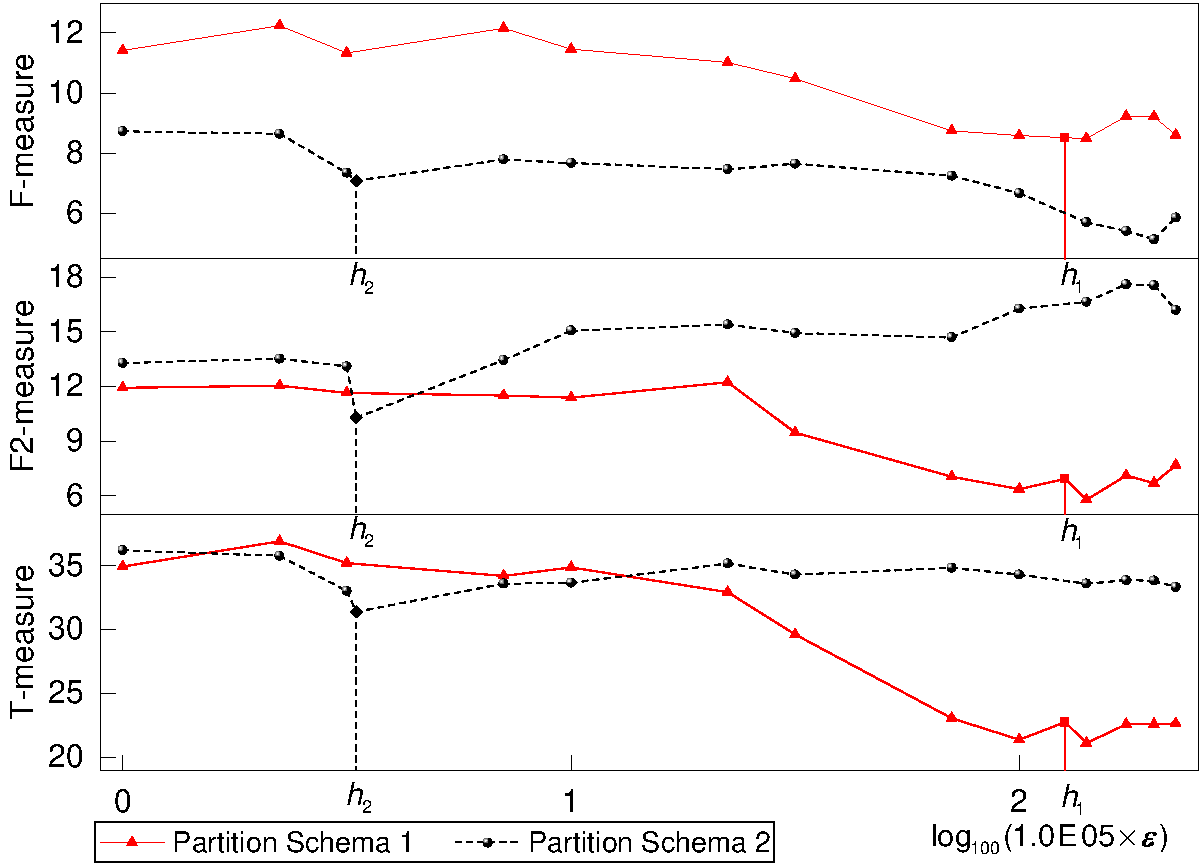
\includegraphics[width=0.32\textwidth,height=5cm]{fig/drtparemeter/avia.pdf}}
	\subfigure[CUBS] {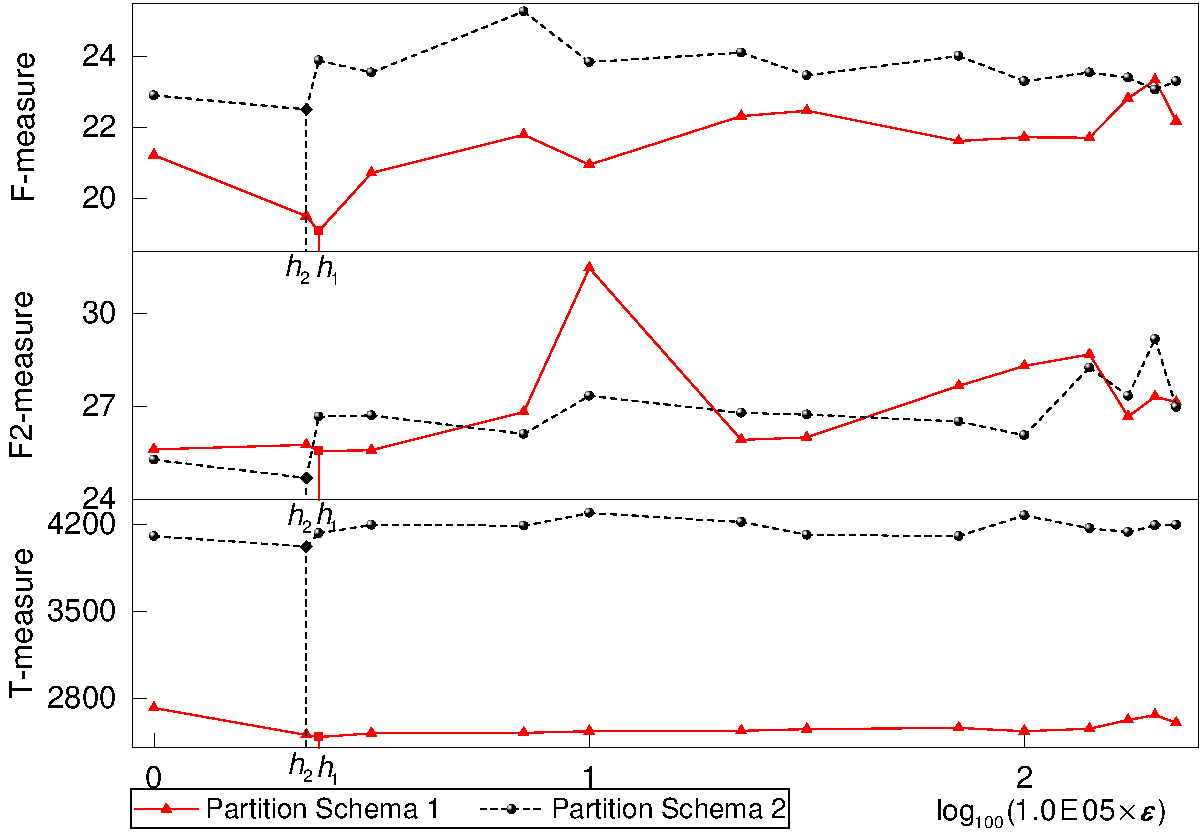
\includegraphics[width=0.32\textwidth,height=5cm]{fig/drtparemeter/china.pdf}}
	\subfigure[PBS] {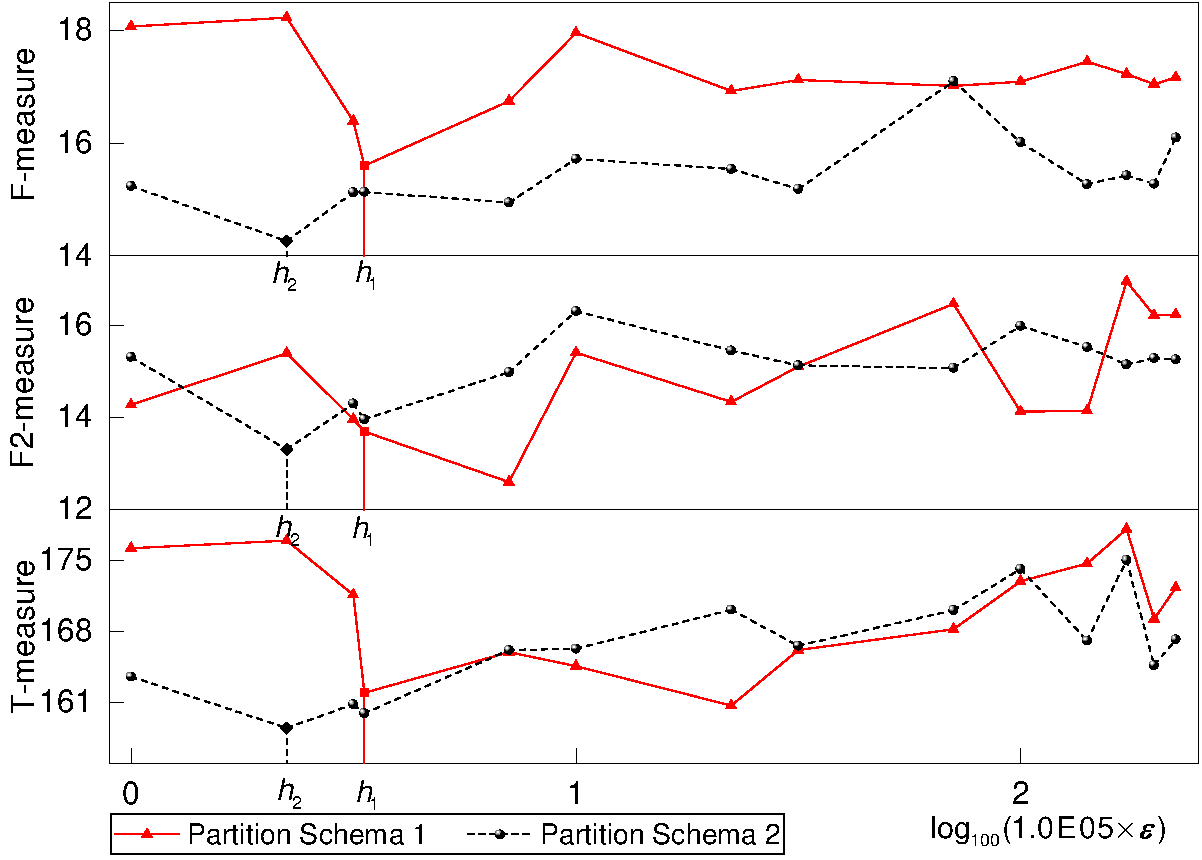
\includegraphics[width=0.32\textwidth,height=5cm]{fig/drtparemeter/parking.pdf}}
	\caption{line charts of F-measure, F2-measure, and T-measure on each object program with theoretical parameter and nontheoretical parameter}
	\label{fig:theovsnontheo}
\end{figure*}
%
%\begin{figure*}
%	\centering
%	\subfigure[ACMS] {\includegraphics[width=0.32\textwidth,height=4cm]{fig//f2aviavsnot}}
%	\subfigure[CUBS] {\includegraphics[width=0.32\textwidth,height=4cm]{fig//f2chinavsnot}}
%	\subfigure[PBS] {\includegraphics[width=0.32\textwidth,height=4cm]{fig//f2parkingvsnot}}
%	\caption{Boxplots of F2-measure on each object program with theoretical parameter}
%	\label{fig:F2theovs}
%\end{figure*}
%
%\begin{figure*}
%	\centering
%	\subfigure[ACMS] {\includegraphics[width=0.32\textwidth,height=4cm]{fig//taviavsnot}}
%	\subfigure[CUBS] {\includegraphics[width=0.32\textwidth,height=4cm]{fig//tchinavsnot}}
%	\subfigure[PBS] {\includegraphics[width=0.32\textwidth,height=4cm]{fig//tparkingvsnot}}
%	\caption{Boxplots of T-measure on each object program with theoretical parameter}
%	\label{fig:Ttheovs}
%\end{figure*}

\subsection{RQ3: Selection Overhead}

Tables~\ref{tab:timeavia} to~\ref{tab:timeparking} summarize the experimental results of F-time, F2-time, and T-time, respectively. The results of distribution on every web services are showed in Figures~\ref{fig:Ftime} to \ref{fig:Ttime}. From Figures~\ref{fig:Ftime} to \ref{fig:Ttime}, we can observe that in general, DRT had the best performance, and RPT just marginally outperformed RT in terms of F-time, F2-time, and T-time.

\begin{table}[!hbt]
  \caption{F-time, F2-time and T-time on web service ACMS (in ms)}
  \label{tab:timeavia}
  \centering
  \setlength{\tabcolsep}{1mm}{
  \begin{tabular}{|c|c|c|c|c|c|c|c|} \hline
     \multicolumn{2}{|c|}{\multirow{2}{*}{Strategy}} &\multicolumn{3}{|c|}{Partition Schema 1} &\multicolumn{3}{|c|}{Partition Schema 2}\\ \cline{3-8}
     \multicolumn{2}{|c|}{}    &F-time	&F2-time &T-time &F-time &F2-time &T-time  \\ \hline
     \multicolumn{2}{|c|}{RT}  &0.43	&0.29	&0.85	&0.43 	&0.29	&0.85   \\ \hline
     \multicolumn{2}{|c|}{RPT} &0.57	&0.31	&1.08	&0.33	&0.45	&0.78   \\ \hline
         \multirow{13}{*}{DRT} &1.0E-5    &0.47	&0.28	&0.96	&0.38	&0.41	&0.95  \\ \cline{2-8}
                               &5.0E-5	  &0.35	&0.21	&0.78	&0.30	&0.27	&0.71 \\ \cline{2-8}
                               &1.0E-4	  &0.33	&0.19	&0.66	&0.24	&0.28	&0.65 \\ \cline{2-8}
                               &5.0E-4	  &0.30	&0.17	&0.60	&0.27	&0.25	&0.67 \\ \cline{2-8}
                               &1.0E-3	  &0.29	&0.19	&0.61	&0.22	&0.24	&0.60 \\ \cline{2-8}
                               &5.0E-3	  &0.28	&0.23	&0.62	&0.21	&0.31	&0.64 \\ \cline{2-8}
                               &1.0E-2	  &0.24	&0.17	&0.53	&0.23	&0.29	&0.66 \\ \cline{2-8}
                               &5.0E-2	  &0.28	&0.13	&0.49	&0.23	&0.35	&0.71 \\ \cline{2-8}
                               &1.0E-1	  &0.26	&0.08	&0.43	&0.23	&0.29	&0.63 \\ \cline{2-8}
                               &2.0E-1	  &0.23	&0.12	&0.43	&0.30	&0.46	&0.89 \\ \cline{2-8}
                               &3.0E-1	  &0.24	&0.11	&0.45	&0.18	&0.40	&0.69 \\ \cline{2-8}
                               &4.0E-1	  &0.27	&0.10	&0.47	&0.16	&0.31	&0.58 \\ \cline{2-8}
                               &5.0E-1	  &0.28	&0.11	&0.47	&0.28	&0.45	&0.86 \\ \hline
  \end{tabular}}
\end{table}


\begin{table}[!hbt]
  \caption{F-time, F2-time and T-time on web service CUBS (in ms)}
  \label{tab:timechina}
  \centering
  \setlength{\tabcolsep}{1mm}{
  \begin{tabular}{|c|c|c|c|c|c|c|c|} \hline
     \multicolumn{2}{|c|}{\multirow{2}{*}{Strategy}} &\multicolumn{3}{|c|}{Partition Schema 1} &\multicolumn{3}{|c|}{Partition Schema 2}\\ \cline{3-8}
     \multicolumn{2}{|c|}{}    &F-time	&F2-time &T-time &F-time &F2-time &T-time  \\ \hline
     \multicolumn{2}{|c|}{RT}  &0.82	&1.14	&34.69	&0.82	&1.14	&34.69   \\ \hline
     \multicolumn{2}{|c|}{RPT} &0.91	&0.87	&30.54	&0.75	&0.79	&34.59   \\ \hline
         \multirow{13}{*}{DRT} &1.0E-5    &0.91	&0.87	&30.14	&0.87	&0.83	&36.49  \\ \cline{2-8}
                               &5.0E-5	  &0.95	&0.86	&30.21	&0.82	&0.75	&34.7\\ \cline{2-8}
                               &1.0E-4	  &0.77	&0.89	&29.27	&0.86	&0.69	&35.34 \\ \cline{2-8}
                               &5.0E-4	  &0.79	&1.00	&31.05	&0.87	&0.90	&36.85 \\ \cline{2-8}
                               &1.0E-3	  &0.86	&0.88	&29.93	&0.92	&0.77	&36.44 \\ \cline{2-8}
                               &5.0E-3	  &0.86	&0.83	&30.28	&0.83	&0.83	&36.27 \\ \cline{2-8}
                               &1.0E-2	  &0.95	&0.88	&29.33	&0.84	&0.72	&35.23 \\ \cline{2-8}
                               &5.0E-2	  &0.84	&0.82	&30.56	&0.88	&0.72	&37.07 \\ \cline{2-8}
                               &1.0E-1	  &0.88	&0.93	&29.45	&0.82	&0.76	&37.14 \\ \cline{2-8}
                               &2.0E-1	  &0.83	&0.83	&30.16	&0.86	&0.73	&36.79 \\ \cline{2-8}
                               &3.0E-1	  &0.95	&0.86	&27.81	&0.84	&0.84	&36.89 \\ \cline{2-8}
                               &4.0E-1	  &0.84	&0.84	&28.23	&0.86	&0.82	&35.22 \\ \cline{2-8}
                               &5.0E-1	  &0.87	&0.84	&27.91	&0.90	&0.86	&38.21 \\ \hline
  \end{tabular}}
\end{table}


\begin{table}[!hbt]
  \caption{F-time, F2-time and T-time on web service PBS (in ms)}
  \label{tab:timeparking}
  \centering
  \setlength{\tabcolsep}{1mm}{
  \begin{tabular}{|c|c|c|c|c|c|c|c|} \hline
     \multicolumn{2}{|c|}{\multirow{2}{*}{Strategy}} &\multicolumn{3}{|c|}{Partition Schema 1} &\multicolumn{3}{|c|}{Partition Schema 2}\\ \cline{3-8}
     \multicolumn{2}{|c|}{}    &F-time	&F2-time &T-time &F-time &F2-time &T-time  \\ \hline
     \multicolumn{2}{|c|}{RT}  &0.81	&0.42	&4.12	&0.81	&0.42	&4.12   \\ \hline
     \multicolumn{2}{|c|}{RPT} &0.85	&0.52	&3.83	&0.66	&0.35	&2.98   \\ \hline
         \multirow{13}{*}{DRT} &1.0E-5    &0.76	&0.48	&3.85	&1.05	&0.51	&3.44  \\ \cline{2-8}
                               &5.0E-5    &0.73	&0.35	&3.02	&0.91	&0.52	&3.79\\ \cline{2-8}
                               &1.0E-4    &0.54	&0.36	&2.97	&0.49	&0.34	&2.26 \\ \cline{2-8}
                               &5.0E-4    &0.68	&0.34	&3.20	&0.50	&0.30	&2.31 \\ \cline{2-8}
                               &1.0E-3    &0.62	&0.38	&2.87	&0.52	&0.38	&2.42 \\ \cline{2-8}
                               &5.0E-3    &0.60	&0.38	&2.99	&0.43	&0.51	&2.40 \\ \cline{2-8}
                               &1.0E-2    &0.58	&0.42	&2.84	&0.51	&0.34	&2.41 \\ \cline{2-8}
                               &5.0E-2    &0.64	&0.44	&3.27	&0.59	&0.36	&2.49 \\ \cline{2-8}
                               &1.0E-1    &0.65	&0.38	&3.46	&0.60	&0.38	&2.56 \\ \cline{2-8}
                               &2.0E-1	  &0.60	&0.36	&3.22	&0.54	&0.59	&2.47 \\ \cline{2-8}
                               &3.0E-1	  &0.59	&0.44	&3.24	&0.57	&0.46	&2.57 \\ \cline{2-8}
                               &4.0E-1	  &0.61	&0.33	&2.90	&0.51	&0.33	&2.54 \\ \cline{2-8}
                               &5.0E-1	  &0.62	&0.44	&3.16	&0.56	&0.36	&2.56 \\ \hline
  \end{tabular}}
\end{table}

\begin{figure*}
	\centering
    \subfigure[ACMS] {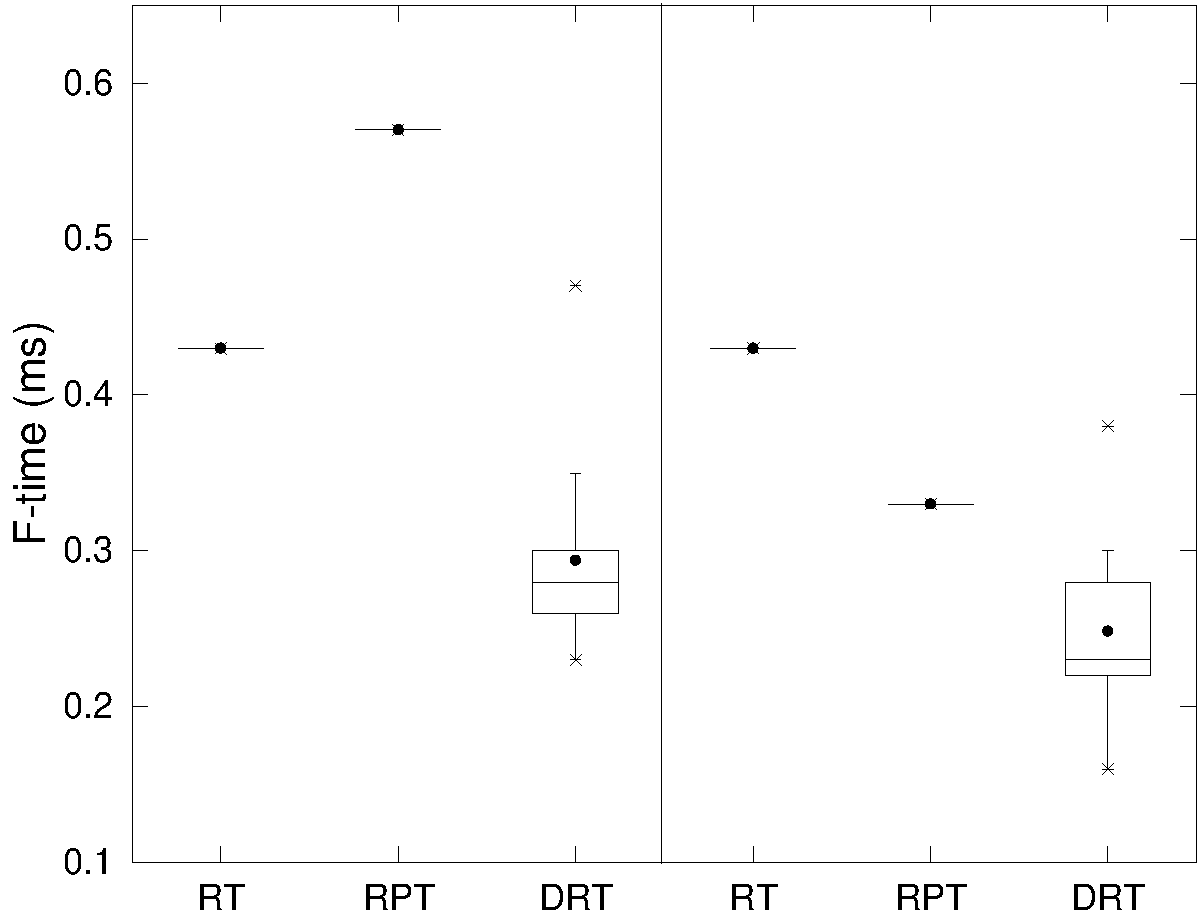
\includegraphics[width=0.32\textwidth,height=4cm]{fig/drttime/aviatimef}}
	\subfigure[CUBS] {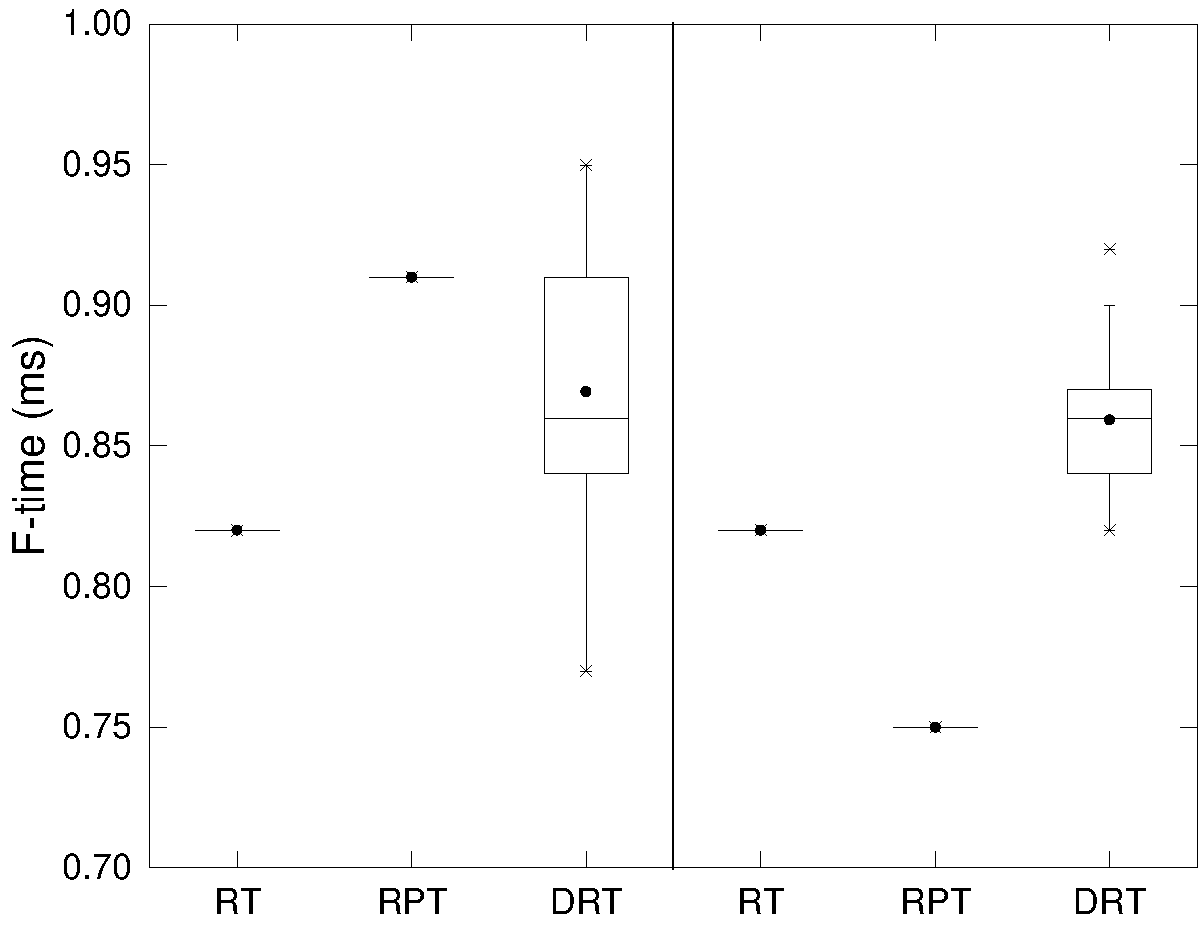
\includegraphics[width=0.32\textwidth,height=4cm]{fig/drttime/chinatimef}}
	\subfigure[PBS] {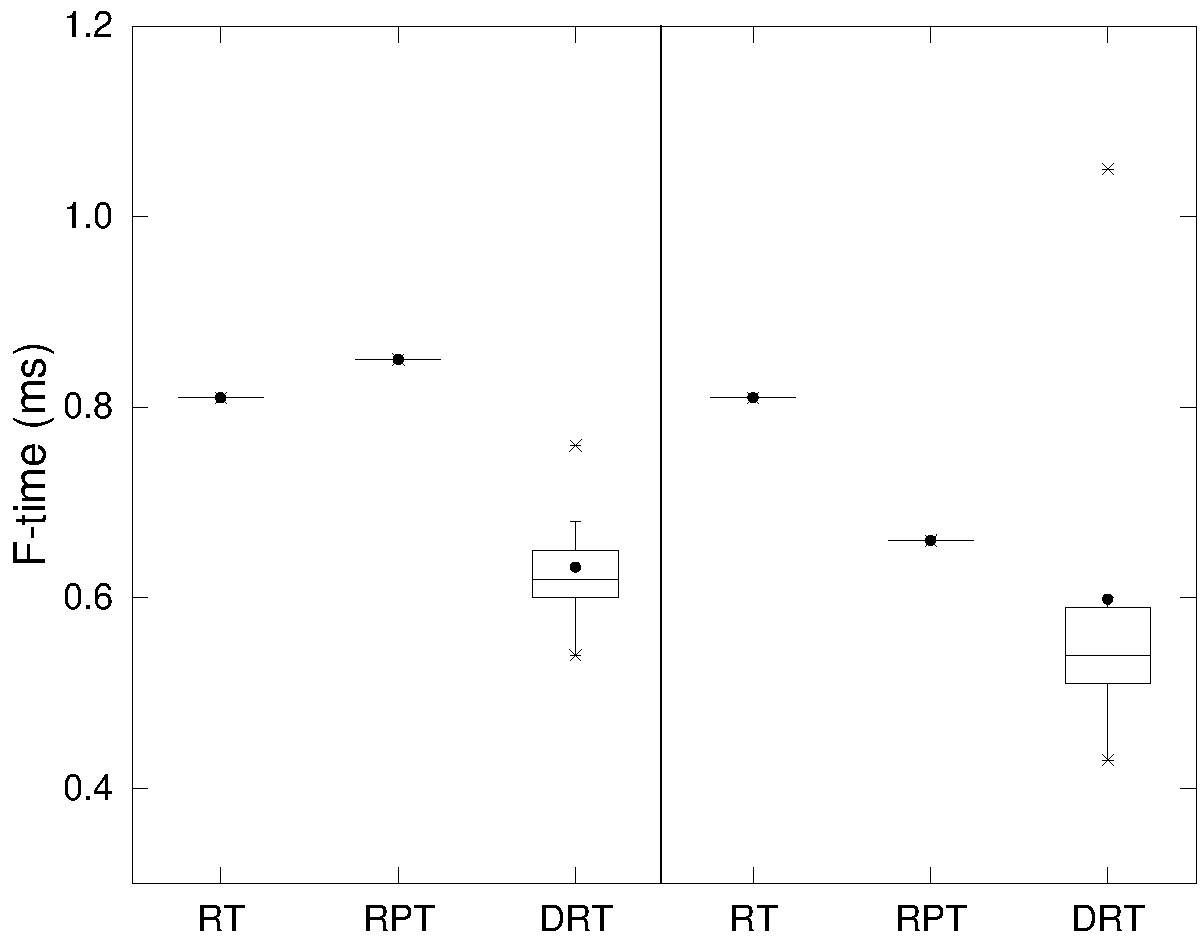
\includegraphics[width=0.32\textwidth,height=4cm]{fig/drttime/parkingtimef}}

	\caption{Boxplots of F-time on each object program}
	\label{fig:Ftime}
\end{figure*}

\begin{figure*}
	\centering
	\subfigure[ACMS] {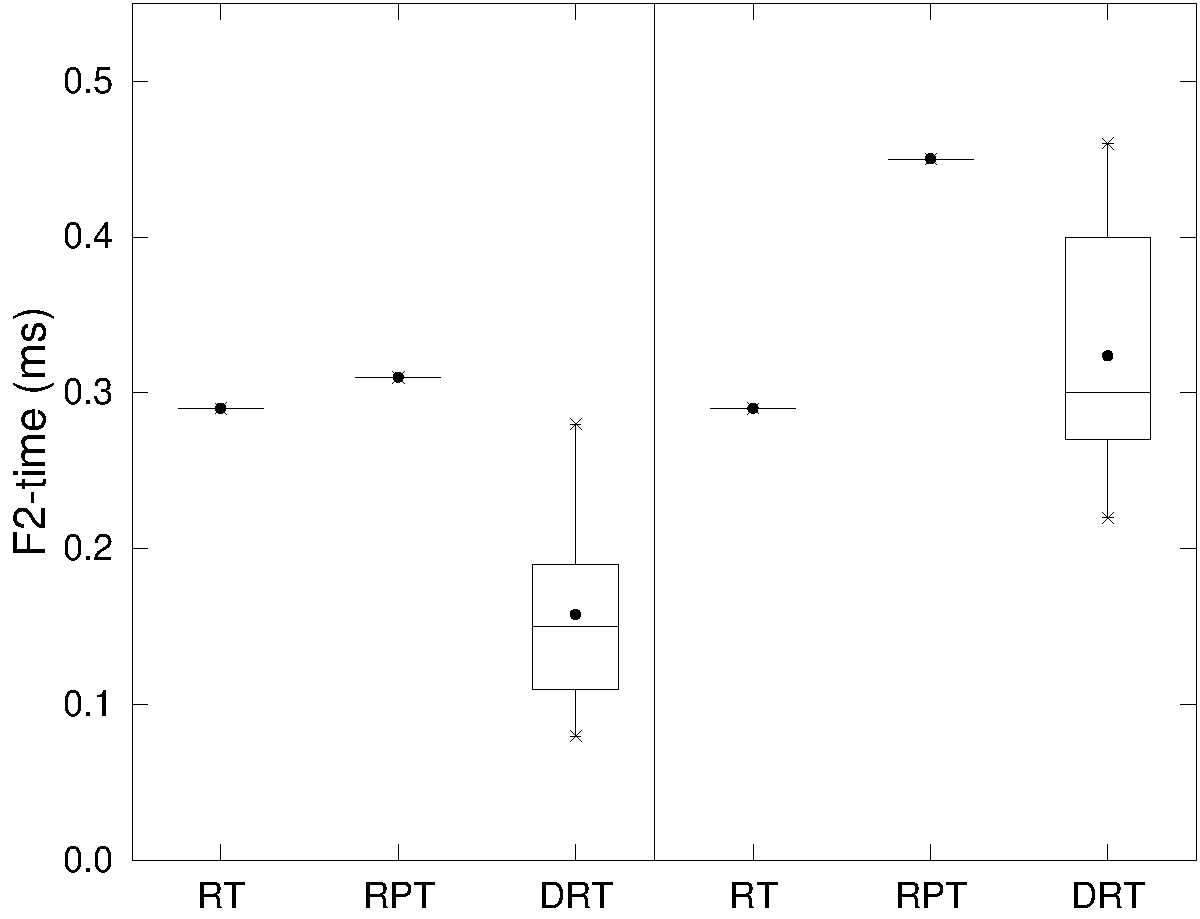
\includegraphics[width=0.32\textwidth,height=4cm]{fig/drttime/aviatimef2}}
	\subfigure[CUBS] {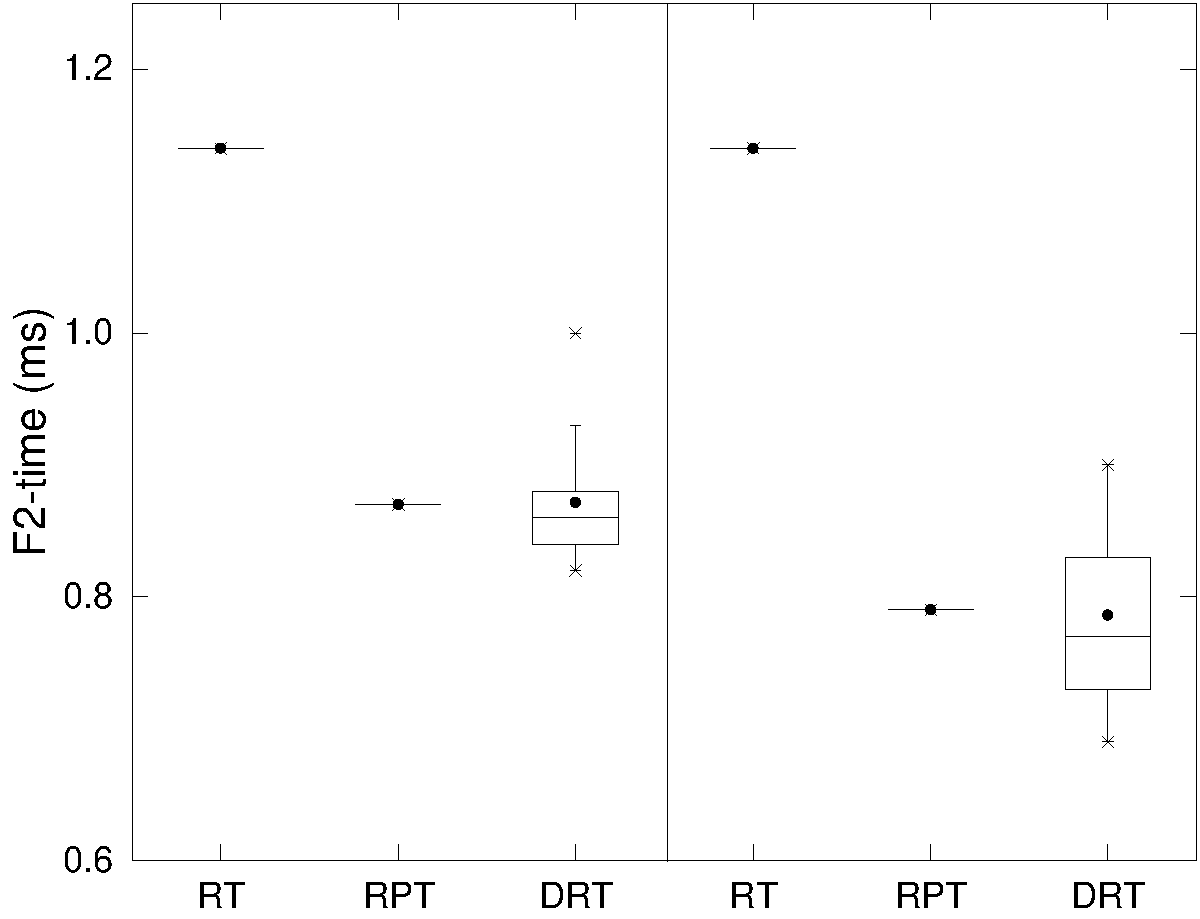
\includegraphics[width=0.32\textwidth,height=4cm]{fig/drttime/chinatimef2}}
	\subfigure[PBS] {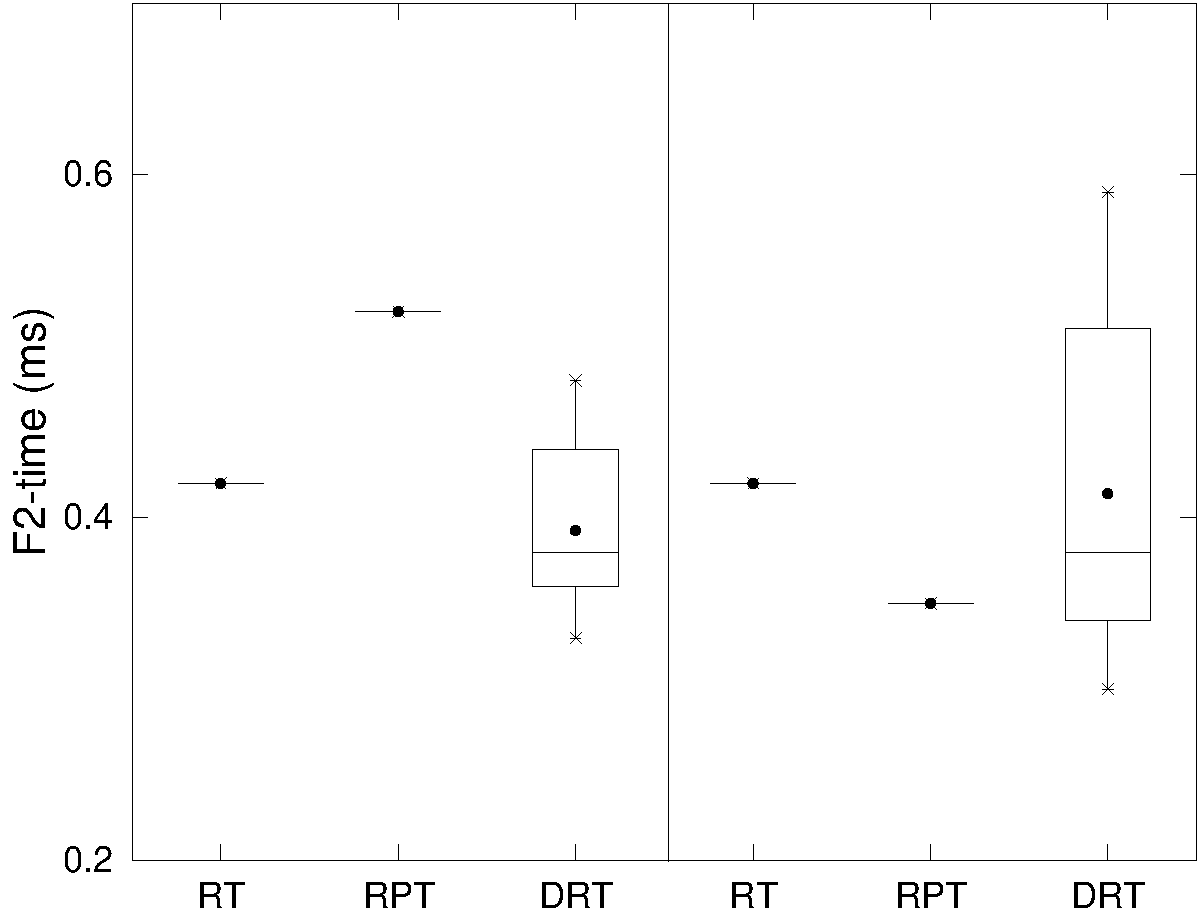
\includegraphics[width=0.32\textwidth,height=4cm]{fig/drttime/parkingtimef2}}
	\caption{Boxplots of F2-time on each object program}
	\label{fig:F2time}
\end{figure*}


\begin{figure*}
	\centering
	\subfigure[ACMS] {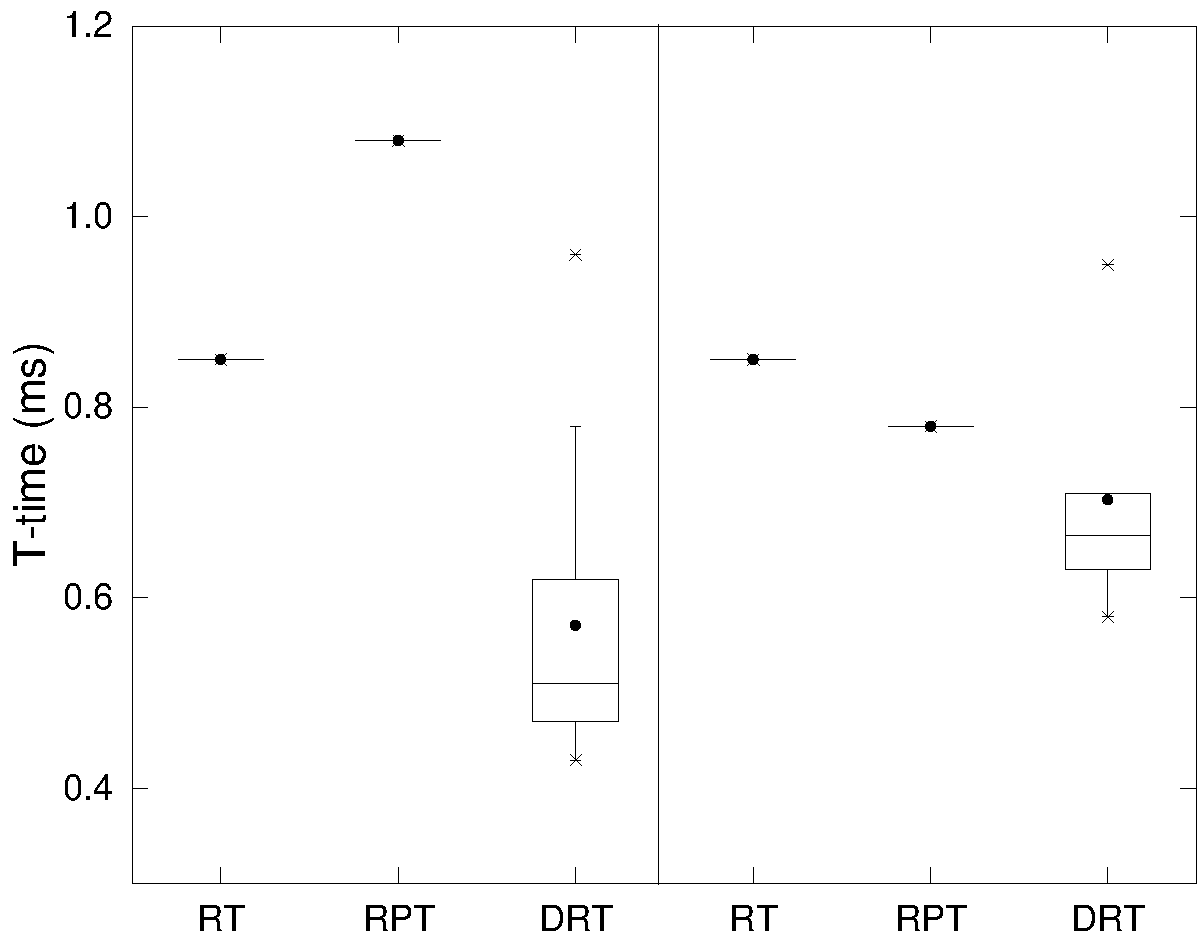
\includegraphics[width=0.32\textwidth,height=4cm]{fig/drttime/aviatimet}}
	\subfigure[CUBS] {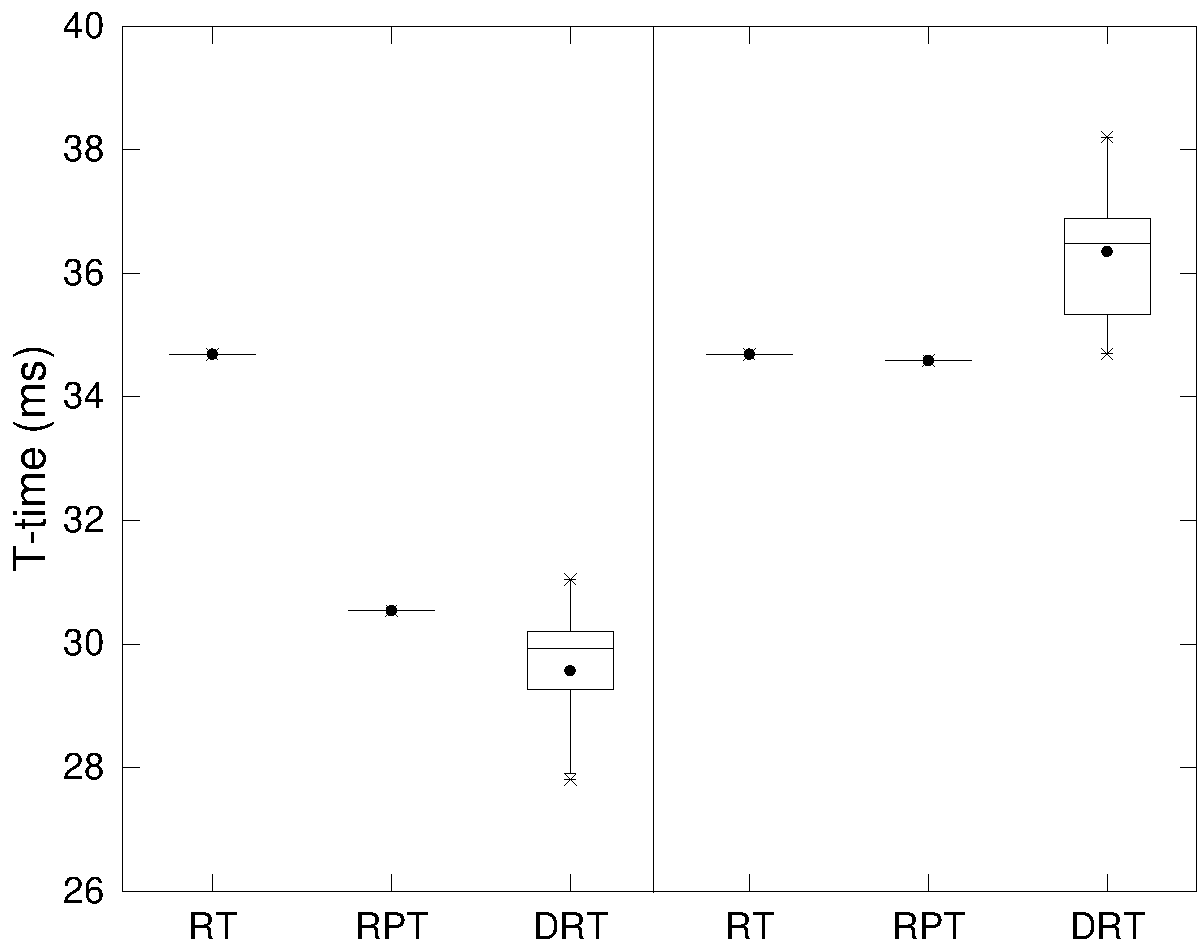
\includegraphics[width=0.32\textwidth,height=4cm]{fig/drttime/chinatimet}}
	\subfigure[PBS] {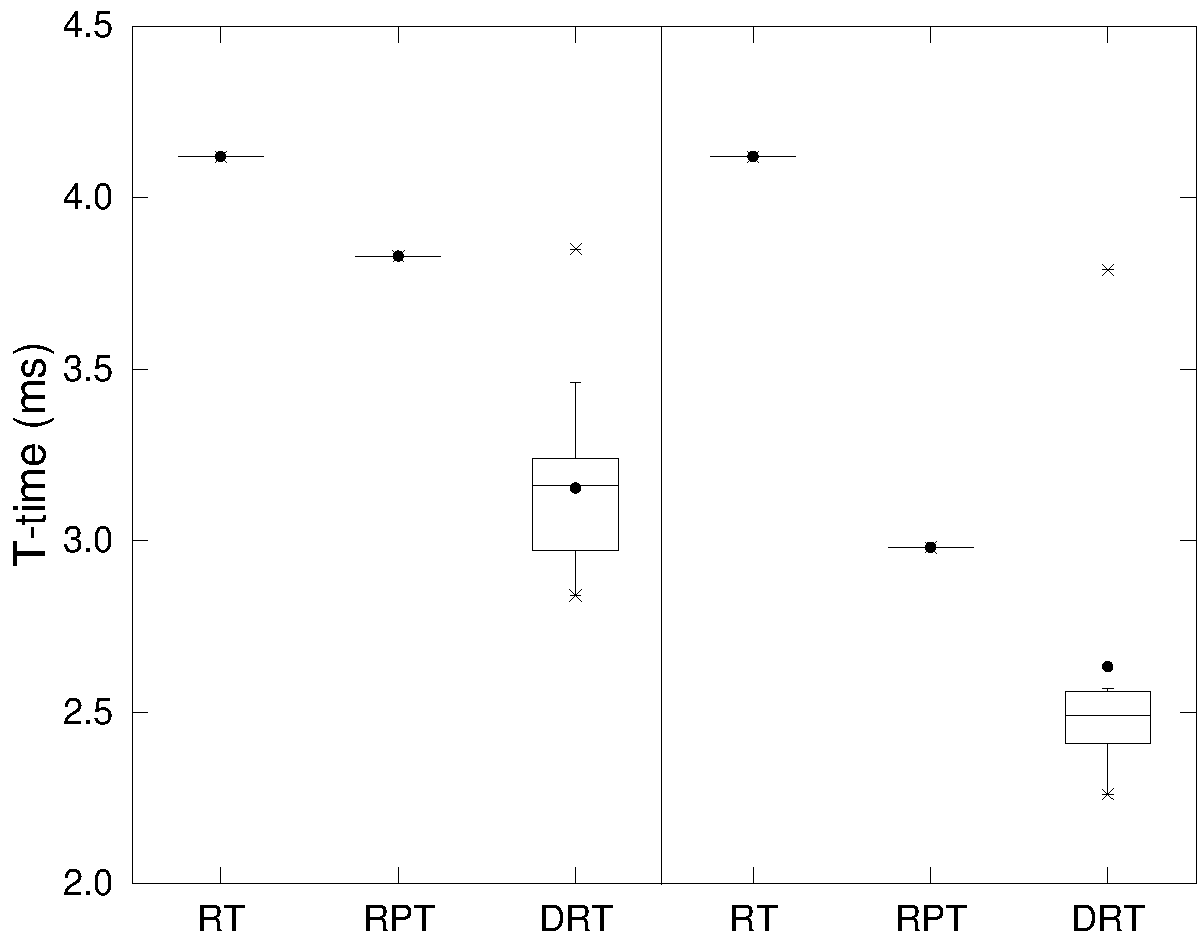
\includegraphics[width=0.32\textwidth,height=4cm]{fig/drttime/parkingtimet}}
	\caption{Boxplots of T-time on each object program}
	\label{fig:Ttime}
\end{figure*}

Similar to the F-measure, F2-measure, and T-measure, we use the Holm-Bonferroni method to check the different between each pair of testing strategies in terms of F-time, F2-time, and T-time, showing in Tables~\ref{tableHolm:ftime} to \ref{tableHlom:ttime}.

From Table \ref{tableHlom:ttime}, we can observe that six entries ("73" \& "3" for DRT vs. RT, "58" vs. "20") are in bold font. There observations imply that in terms of T-time, DRT was significantly better than RT and DRT only marginally outperformed RPT. Similar observation was made on the results of F-time and F2-time. In other words, the additional computation incurred in DRT for updating the test profile is compensated with the saving of test executions.

\begin{table}[!htbp]
  \caption{Number of scenarios where the technique on top row has smaller F-time than that on left column}
  \centering
  \label{tableHolm:ftime}
  \begin{tabular}{|c|c|c|c|} \hline
          &RT         &RPT         &DRT         \\ \hline
    RT    & ---       &5           &\textbf{62} \\ \hline
    RPT   &1          & ---        &\textbf{47} \\ \hline
    DRT   &\textbf{16}&\textbf{31} & ---        \\ \hline
  \end{tabular}
\end{table}

\begin{table}[!htbp]
  \caption{Number of scenarios where the technique on top row has smaller F2-time than that on left column}
  \centering
  \label{tableHlom:nftime}
  \begin{tabular}{|c|c|c|c|} \hline
          &RT         &RPT         &DRT         \\ \hline
    RT    & ---       &3           &\textbf{52} \\ \hline
    RPT   &3          & ---        &\textbf{48} \\ \hline
    DRT   &\textbf{26} &\textbf{30}& ---         \\ \hline
  \end{tabular}
\end{table}

\begin{table}[!htbp]
  \caption{Number of scenarios where the technique on top row has smaller T-time than that on left column}
  \centering
  \label{tableHlom:ttime}
  \begin{tabular}{|c|c|c|c|} \hline
          &RT         &RPT         &DRT         \\ \hline
    RT    & ---       &5           &\textbf{73} \\ \hline
    RPT   &1          & ---        &\textbf{58} \\ \hline
    DRT   &\textbf{3} &\textbf{20} & ---         \\ \hline
  \end{tabular}
\end{table}

We can observe that DRT only slightly outperformed RPT from Tables~\ref{tableHolm:ftime} to \ref{tableHlom:ttime}, but DRT is significantly better than RT especially in term of $T$-$time$.

In short, DRT strategy was considered as the best testing technique across all six metrics, and RPT was marginally outperformed RT.

\section{Related Work}
\label{sec:relatedwork}

In this section, we describe related work in two dimensions, one is related to testing techniques for web services, and the other is related to improvements on RT and PT.

\subsection{Testing Techniques for Web Services}

In recent years, many efforts have been made to test web services~\cite{canfora2006service, bozkurt2010}. Test case generation that includes generating and selecting test cases, is core procedure to test web services. Model-based~\cite{dalal1999model} and specification-based techniques are two common test case generation methods. Before service providers put services on Internet, testers can use model-based technique to verify whether the behaviors of WSUT meet their requirements. In this technique, test data are generated from a data model that is a specification of the inputs to the software, and can be built before or parallel to the software development process. There are plenty of verification methods using models such as theorem proving, model-checking and Petri-Nets. Sinha et al.~\cite{sinha2006model} generated test cases using theorem proving, where they used of existing test generation methods based on Extended Finite State Machine(EFSM) specification. Majdi et al.~\cite{ghannoudi2015formal} generate test data using model checking. Dong et al.~\cite{dong2006web} combined Hight level Petri-Nets (HPN) with constraint-based test data generation which can get sufficient test data to detect faults. On the other hand, the specification of web service is the only information that users can receive. Therefore, specification-based testing becomes a natural choice. In traditional web service, the specification of web service is named WSDl, and provides information about available operations and its parameters. Many methods proposed for WSDL-based test data generation are based on the XML schema data type. Hanna and Munro proposed a framework that can be used to test the robustness quality attribute of a web service~\cite{hanna2009approach}. This framework is based on analyzing the web service Description Language (WSDL) document of web services to identify what faults could affect the robustness attribute and then test cases were designed to detect those faults.

However, the above approaches aim to generate test cases ignoring the impact of the execution order of test cases on test efficiency.
Askarunisa et al.~\cite{Askarunisa2011prioritization} performed prioritization of test cases based on various coverage criteria for composite web services. The major drawback of this approach is that it takes extra time to sort the test cases before starting the test. Bertolino et al.~\cite{bertolino2007automatic} proposed the use of the category-partition method~\cite{Ostrand88} with XML Schemas in order to perform XML-based partition testing.
Partition testing aims to find subsets of the test cases that can adequately test a system. Therefore, partition testing can help in solving one of the major problems of testing high cost by reducing the required number of test cases. Our approach introduce software cybernetics into partition testing. In DRT, the strategy of selecting a partition is according to testing profile, and the testing profile is updated during the test process. The main advantage of DRT is that partitions with larger failure rates have higher selected probability.

Besides, there are some frameworks to illustrate how the test task is completed. Zhu and Zhang~\cite{zhu2012collaborative} proposed a framework of collaborative testing. In this framework, test tasks are completed by collaborating various test services. A test service is a service assigned to perform various test task. This framework focuses on complete test task. However, our framework proposed in section~\ref{sec:framework} aims to find more faults of WSUT. In our framework, the result of current test case execution provides feedback to the control system in order that the next test case selected has a bigger chance to reveal faults of WSUT.

Most existing testing techniques for web services assume that for each test case, the computed output is verifiable. However, the assumption is not always true in practice and thus these testing techniques may be inapplicable in some situations. To address the outstanding oracle problem with testing web services, a metamorphic testing technique was proposed, which not only alleviates the oracle problem, but also presents a feasible and efficient choice for testing web services~\cite{sun2011}.

%The proposed DRT for web services has the following advantages: (1) it is easier to use; (2) it is more efficient because it enhances partition testing with dynamic testing profiles updates and the assocaited overhead is very limited. DRT is applicable whenever partition testing is applicable.

\subsection{Improvement on RT and PT}

Based on the observation that failure causing inputs tend to cluster into contiguous regions within the input domain~\cite{Ammann88, Finelli91}, many works have been done to improve RT. Adaptive random testing~\cite{Chen10} is a family of advanced random testing techniques aims to improve the failure detection effectiveness by evenly spreading test cases executed. The most well-known ART is the Fixed-Size Candidate Set ART technique (FSCS-ART). Others ART algorithms have been developed and their effectivenesses are validated by simulation and experiments~\cite{chen2010adaptive, chen2006impact, barus2016cost}.

Adaptive testing (AT)~\cite{cai2005partition} is based on the same observation, which outperformed both RT and RPT. However, it requires very long execution time in practice. To alleviate this problem, Cai et al. ~\cite{cai2009random} proposed DRT, which uses testing information to dynamically adjust testing profile. There are several aspects that affect the test efficiency of DRT such as testing profile, parameters etc. Yang et al.~\cite{Yang2014Dynamic} proposed A-DRT, which adjusts parameters during testing process. Li et al.~\cite{li2015} developed O-DRT technique, which will change testing profile to a theoretically optimal one when the pre-defined criterion is satisfied. Lv et al.~\cite{Lv2011} studied the relationship of parameters in DRT, but they did not give the relationship between parameters and the number of partitions.



\section{Conclusion}
\label{sec:conclusion}

We have presented a dynamic random testing technique for web services to address the challenges of testing SOA-based applications. The proposed technique employs random testing to generate test cases, and selects test cases for execution from different partitions in accordance with the testing profile of partitions which is dynamically updated in response to the test data collected online. In this way, the proposed test technique takes benefits of both random testing and partition testing.

We proposed a framework which examines key issues when applying DRT to testing web services, and developed a prototype to make the method practically feasible and effective. In order to guide testers properly set parameter of DRT strategy according to concrete testing objects, we use the theoretical analysis approach to get the relationship between number of partitions, parameter of DRT and the failure rates of partitions. Validating the feasibility and effectiveness of our approach, three real web services are used to  experimental objects. The results of empirical study show that in general DRT shows better performance than RT and RPT, and DRT always delivers an outstanding and stable performance in particular when the parameters lie in our theoretically derived interval. In other words, our theoretical analysis can provide a truly useful guidance when DRT is used for different situations.

In our future work, we plan to conduct experiments on more web services to further validate the effectiveness and identify the limitations of our method.

% use section* for acknowledgment
\section*{Acknowledgment}

This research is supported by the National Natural Science Foundation of China under Grant No. 61370061, the Beijing Natural Science Foundation (Grant No. 4162040), the Aeronautical Science Foundation of China (Grant No. 2016ZD74004), and the Fundamental Research Funds for the Central Universities under Grant No. FRF-GF-17-B29.

% Can use something like this to put references on a page
% by themselves when using endfloat and the captionsoff option.
\ifCLASSOPTIONcaptionsoff
  \newpage
\fi


\bibliographystyle{IEEEtran}
\bibliography{DRT4WS}


\begin{IEEEbiography}[{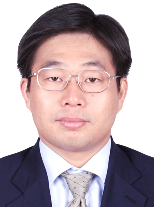
\includegraphics[width=1in,height=1.25in,clip,keepaspectratio]{fig/authers/CASun.pdf}}]{Chang-ai Sun} is a Professor in the School of Computer and Communication Engineering, University of Science and Technology Beijing. Before that, he was an Assistant Professor at Beijing Jiaotong University, China, a postdoctoral fellow at the Swinburne University of Technology, Australia, and a postdoctoral fellow at the University of Groningen, The Netherlands. He received the bachelor degree in Computer Science from the University of Science and Technology Beijing, China, and the PhD degree in Computer Science from the Beihang University, China. His research interests include software testing, program analysis, and Service-Oriented Computing.
\end{IEEEbiography}

%\begin{IEEEbiography}[{\includegraphics[width=1in,height=1.25in,clip,keepaspectratio]{YZhao}}]
\begin{IEEEbiography}[{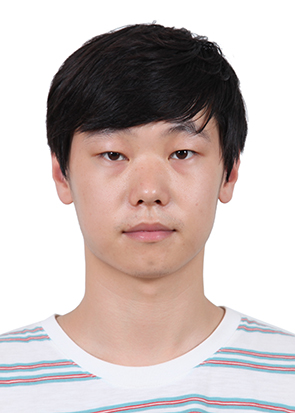
\includegraphics[width=1in,height=1.25in,clip,keepaspectratio]{fig/authers/HPDai_1.jpg}}]{Hepeng Dai} is a PhD student in the School of Computer and Communication Engineering, University of Science and Technology Beijing, China. He received the master degree in Software Engineering from University of Science and Technology Beijing, China and the bachelor degree in Information and Computing Sciences from China University of Mining and Technology, China. His current research interests include software testing and debugging.
\end{IEEEbiography}

%\begin{IEEEbiography}[{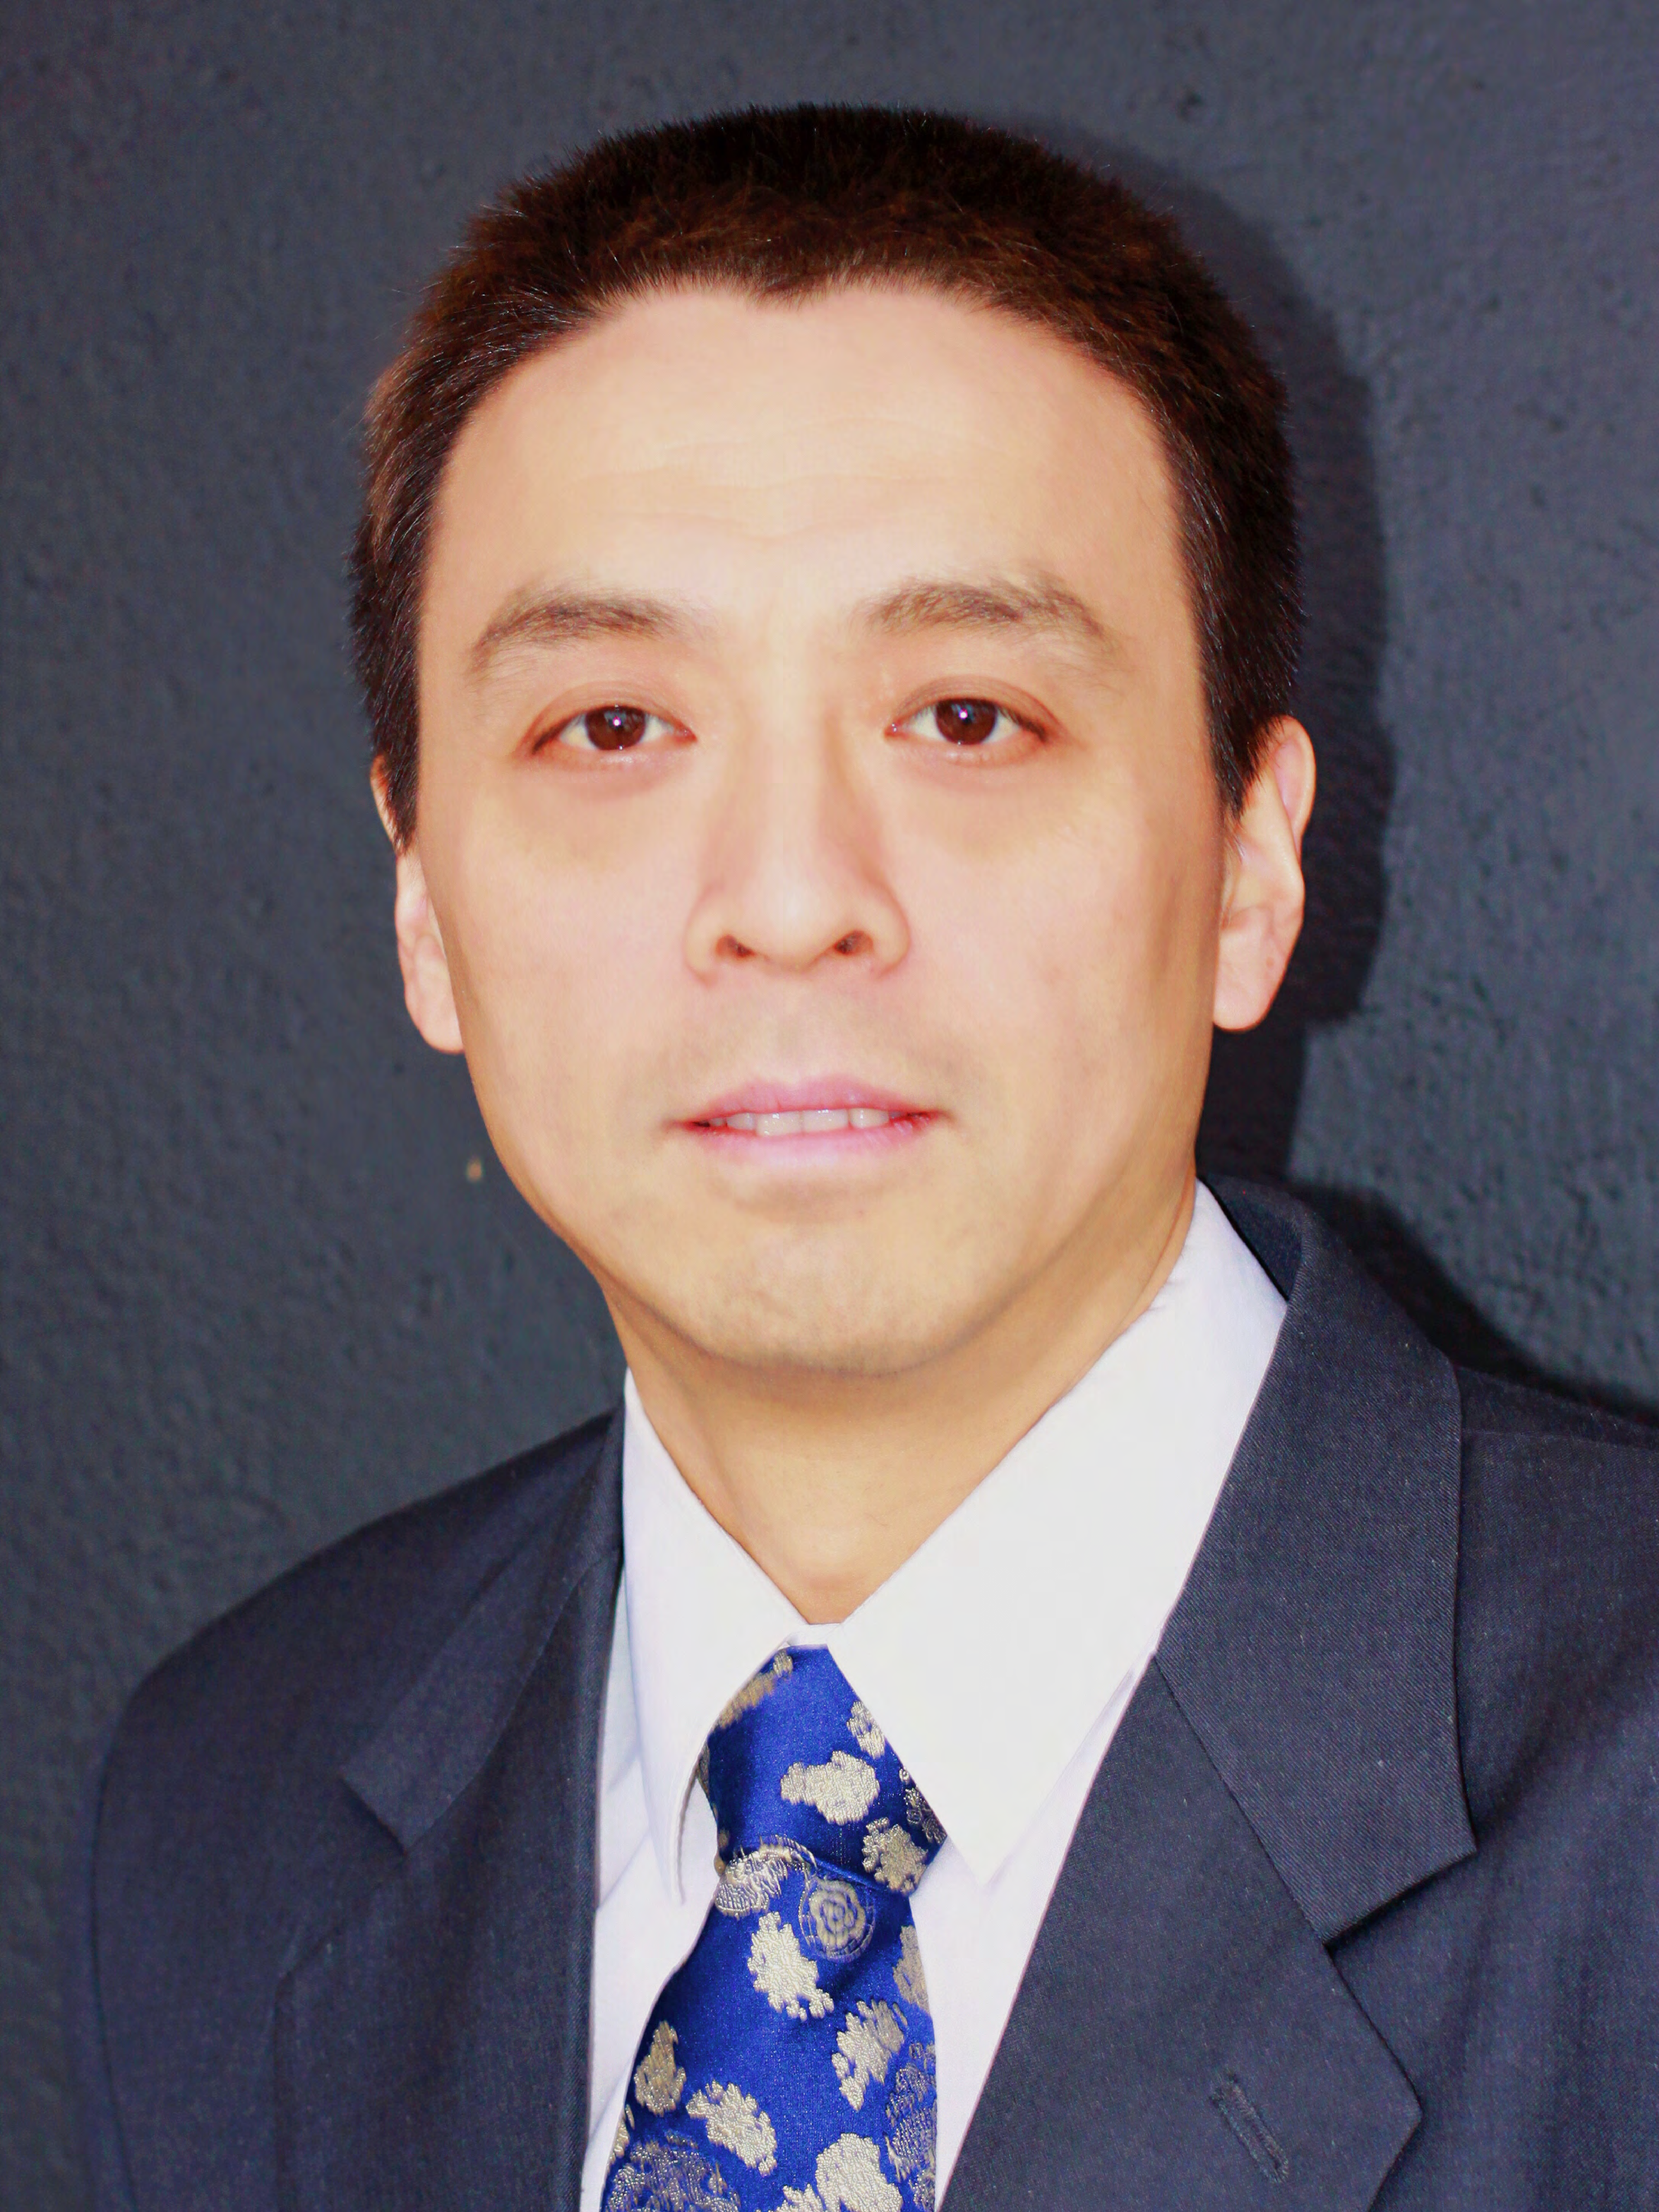
\includegraphics[width=1in,height=1.25in,clip,keepaspectratio]{HLiu}}]
\begin{IEEEbiography}[{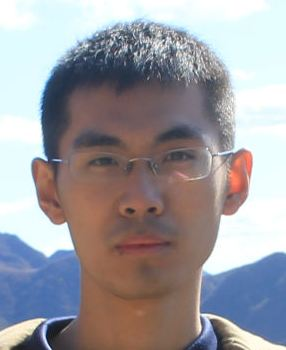
\includegraphics[width=1in,height=1.25in,clip,keepaspectratio]{fig/authers/GWang.jpg}}]{Guan Wang} ig is a master student at the School of Computer and Communication Engineering, University of Science and Technology Beijing. He received a bachelor degree in Computer Science from University of Science and Technology Beijing. His current research interests include software testing and Service-Oriented Computing.
\end{IEEEbiography}

%\begin{IEEEbiography}[{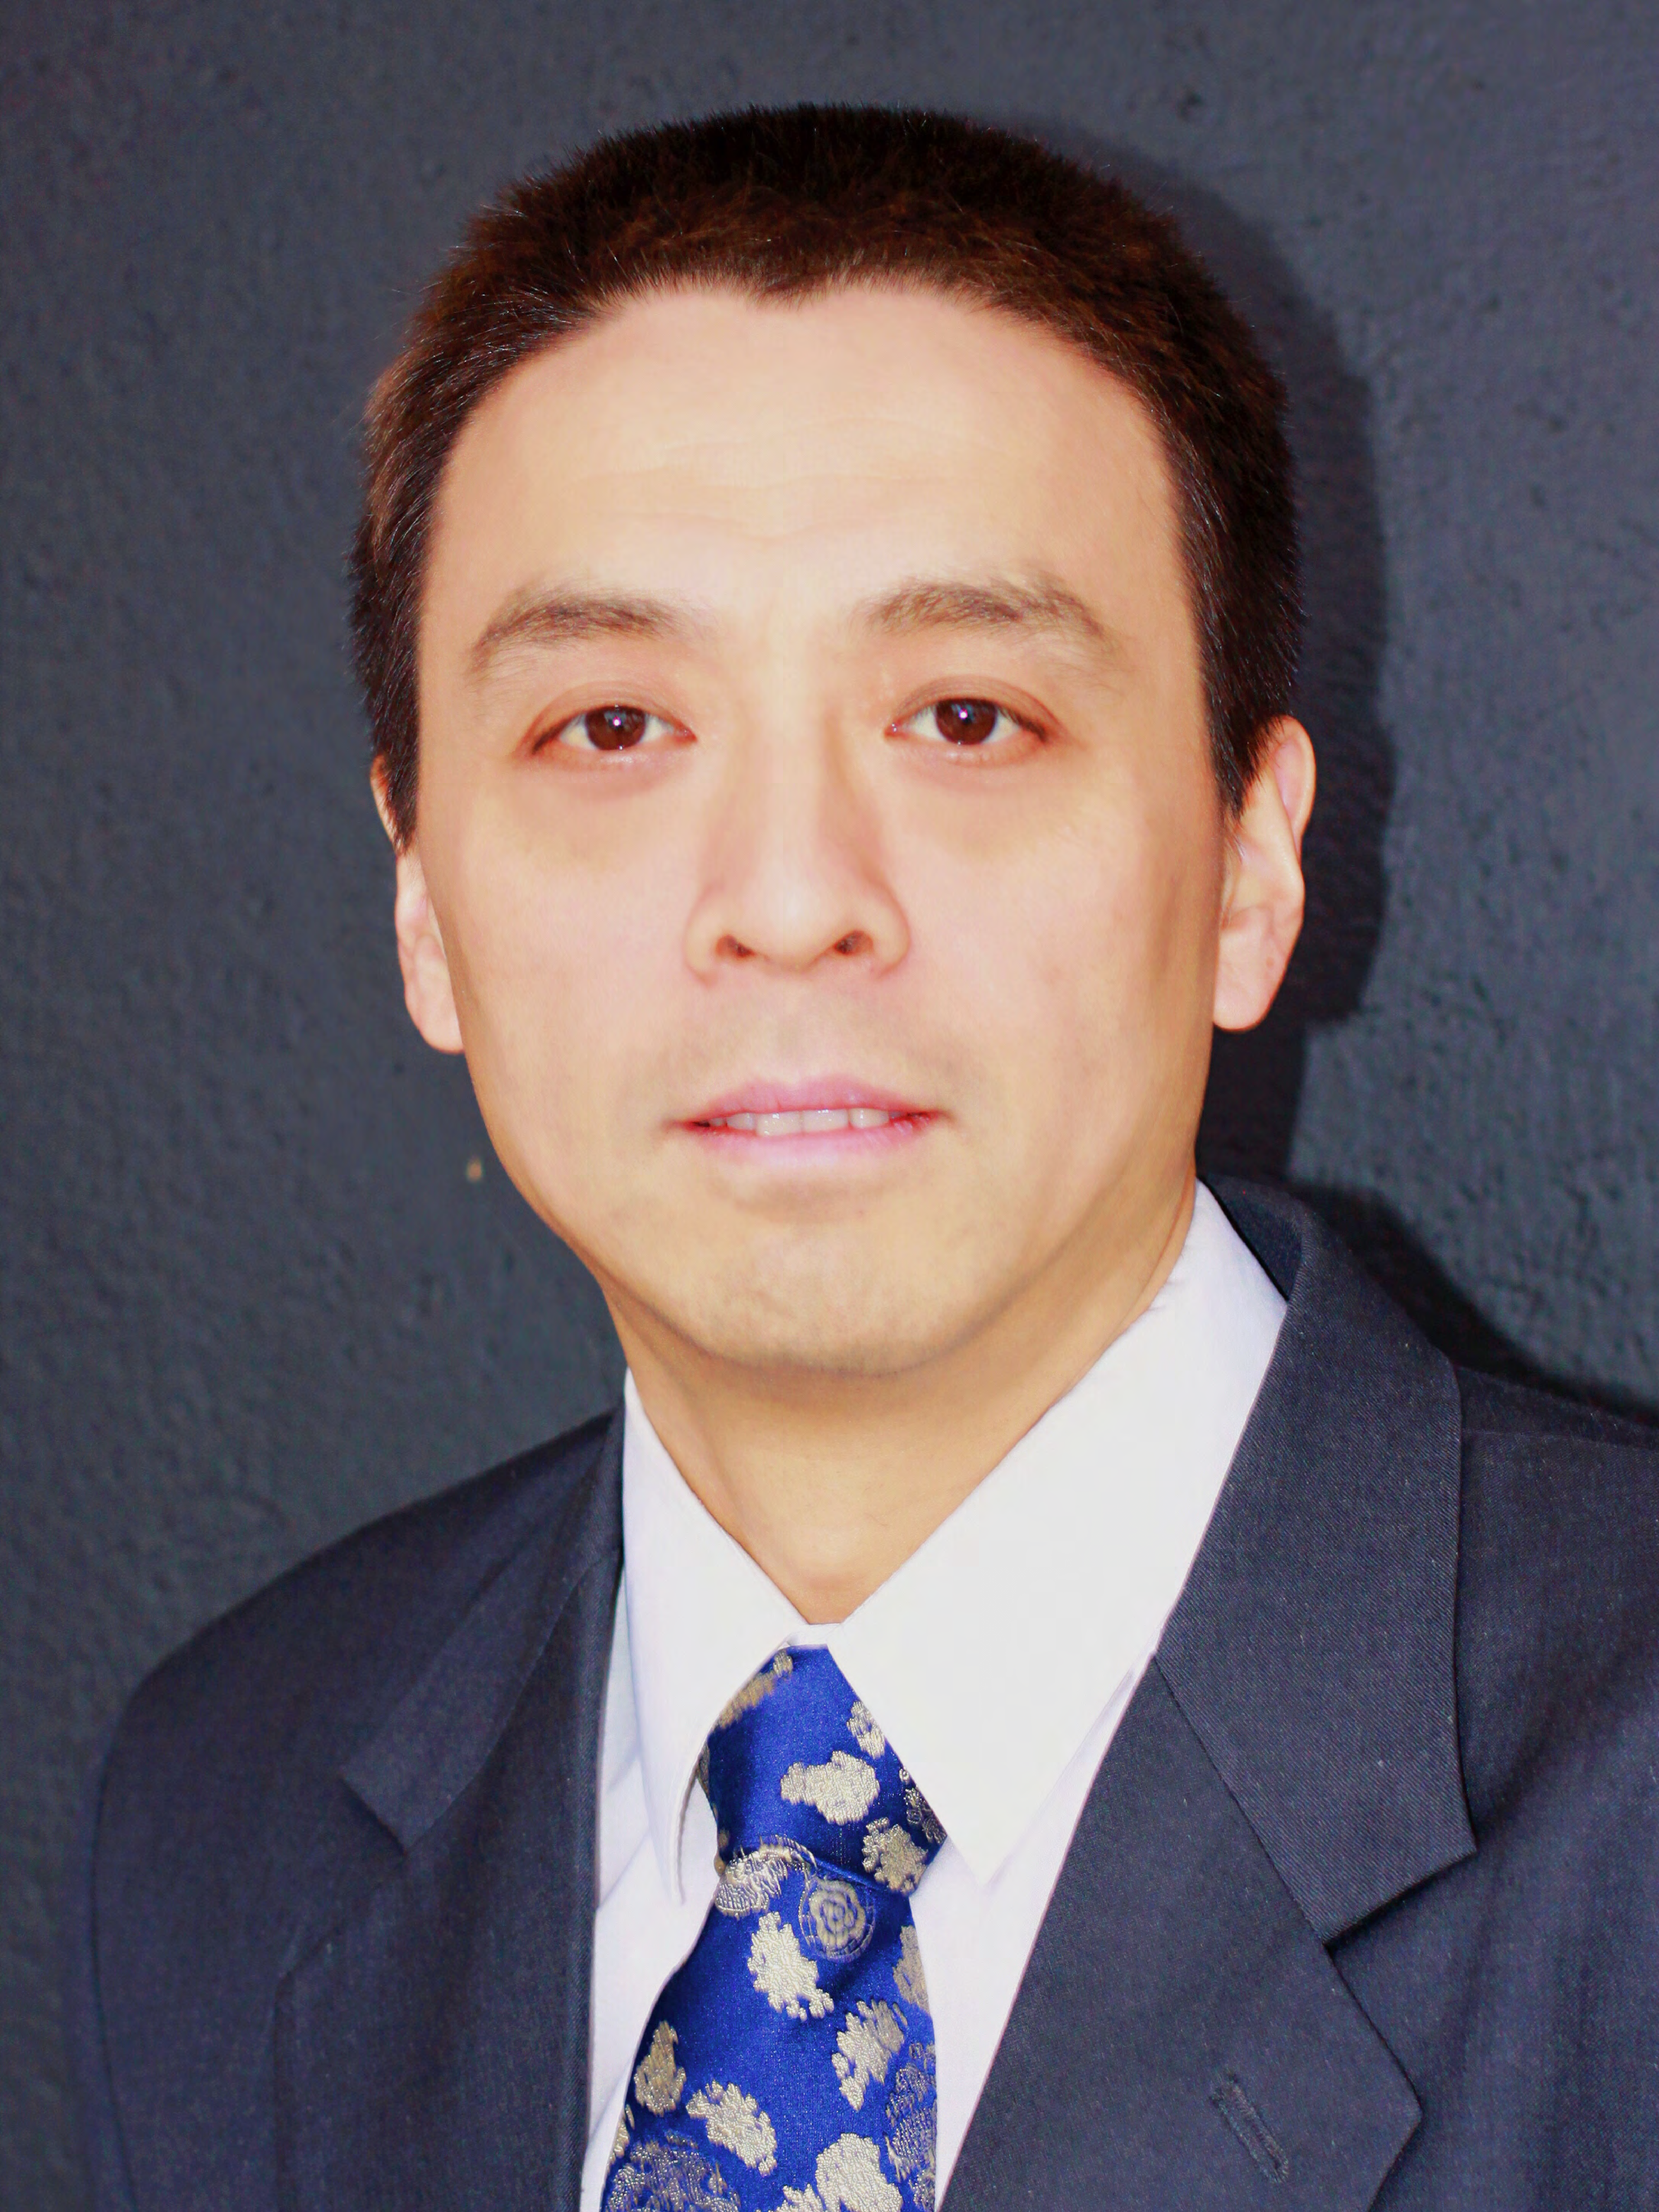
\includegraphics[width=1in,height=1.25in,clip,keepaspectratio]{HLiu}}]
\begin{IEEEbiography}[{
\includegraphics[width=1in,height=1.25in,clip,keepaspectratio]{fig/authers/DTowey.jpg}}]{Dave Towey} is an associate professor in the School of Computer Science, the University of Nottingham Ningbo China. He received his BA and MA degrees from The University of Dublin, Trinity College, PgCertTESOL from The Open University of Hong Kong, MEd from The University of Bristol, and PhD from The University of Hong Kong. His current research interests include technology-enhanced teaching and learning, and software testing, especially metamorphic testing and adaptive random testing.
\end{IEEEbiography}

\begin{IEEEbiography}[{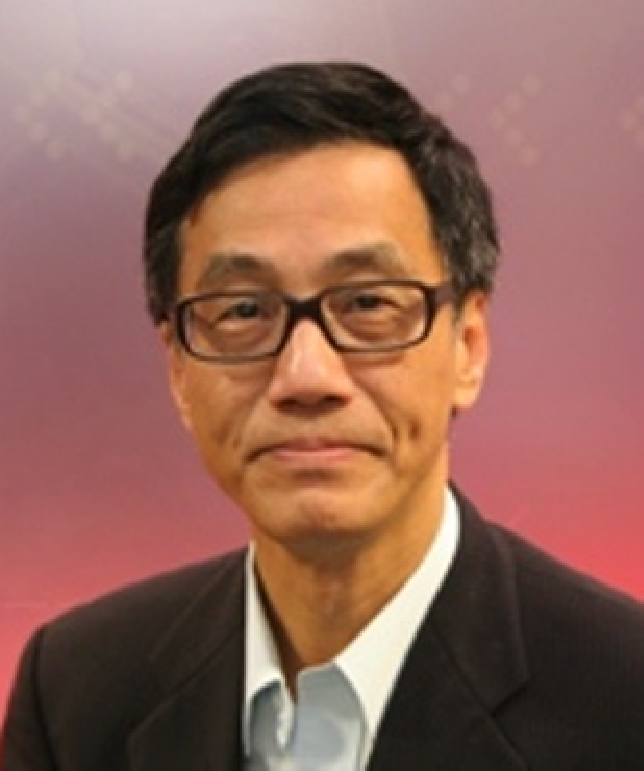
\includegraphics[width=1in,height=1.25in,clip,keepaspectratio]{fig/authers/TYChen.pdf}}]{Tsong Yueh Chen} is a Professor of Software Engineering at the Department of Computer Science and Software Engineering in Swinburne University of Technology. He received his PhD in Computer Science from The University of Melbourne, the MSc and DIC from Imperial College of Science and Technology, and BSc and MPhil from The University of Hong Kong. His current research interests include software testing and debugging, software maintenance, and software design.
\end{IEEEbiography}

%\begin{IEEEbiography}[{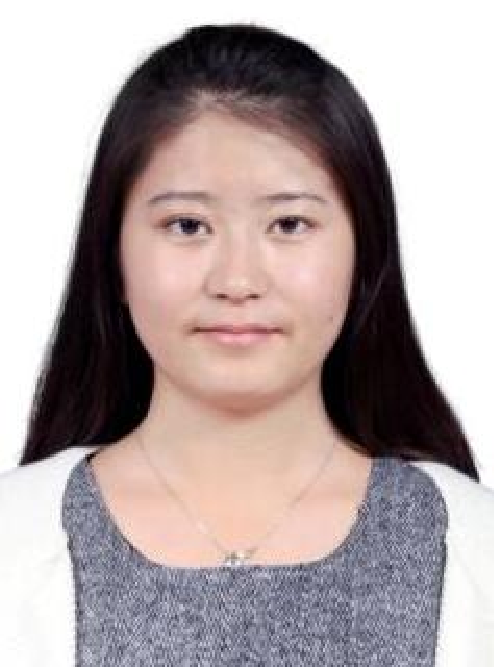
\includegraphics[width=1in,height=1.25in,clip,keepaspectratio]{LPan}}]
\begin{IEEEbiography}[{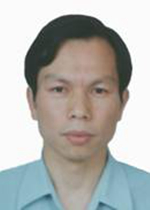
\includegraphics[width=1in,height=1.25in,clip,keepaspectratio]{fig/authers/KYCai.pdf}}]{Kai-Yuan Cai} received the BS, MS, and PhD degrees from Beijing University of Aeronautics and Astronautics, Beijing, China, in 1984, 1987, and 1991, respectively. He has been a full professor at Beihang University since 1995. He is a Cheung Kong Scholar (chair professor), jointly appointed by the Ministry of Education of China and  the Li Ka Shing Foundation of Hong Kong in 1999. His main research interests include software testing, software reliability, reliable flight control, and software cybernatics.
\end{IEEEbiography}


\end{document}
